\PassOptionsToPackage{countmax}{subfloat}
\makeatletter
\def\caption@documentclass{standard}
\makeatother
\documentclass[gmd, manuscript]{copernicus}

\renewcommand{\thesection}{S\arabic{section}}
\renewcommand{\thesubsection}{S\arabic{section}.\arabic{subsection}}
\renewcommand{\thefigure}{S\arabic{figure}}
\renewcommand{\thetable}{S\arabic{table}}

\begin{document}
% Generated from schema-v3/v4 machine artifacts; do not edit by hand.
\newcommand{\ValidationTrials}{300}
\newcommand{\ValidationReferenceRepetitions}{200}
\newcommand{\GaussianCrossingMaximum}{0.0\,\%}
\newcommand{\HeavyTailCrossingRate}{0.3\,\%}
\newcommand{\MultimodalCrossingRate}{0.0\,\%}
\newcommand{\BalancedShiftCrossingRate}{99.3\,\%}
\newcommand{\CfiveLikeShiftCrossingRate}{39.7\,\%}
\newcommand{\MinimumShiftCrossingRate}{32.3\,\%}
\newcommand{\IntervalCoverageMinimum}{91.7\,\%}
\newcommand{\IntervalCoverageMaximum}{95.8\,\%}
\newcommand{\IntervalSeedRepetitions}{24}
\newcommand{\IntervalTargetResamples}{5\,000}
\newcommand{\CorrectBlockReferenceWidth}{0.337}
\newcommand{\FrameIIDReferenceWidth}{0.178}
\newcommand{\GeneratedPerClass}{1\,000}
\newcommand{\GeneratedTotal}{6\,000}
\newcommand{\TrainingFrames}{51\,890}
\newcommand{\TrainingStorms}{2\,761}
\newcommand{\ValidationFrames}{7\,191}
\newcommand{\ValidationStorms}{379}
\newcommand{\TestFrames}{7\,011}
\newcommand{\TestStorms}{368}
\newcommand{\MemorizationTrainingFields}{51\,890}
\newcommand{\ControlReferenceFields}{1\,000}
\newcommand{\CfiveFrames}{85}
\newcommand{\CfiveStorms}{22}
\newcommand{\RealTropicalStormShare}{56.2\,\%}
\newcommand{\RealCategoryFiveShare}{1.2\,\%}
\newcommand{\ControlLaneCount}{17}
\newcommand{\MinimumResolvedCopyFraction}{25\,\%}
\newcommand{\WindSlopeComparisons}{42}
\newcommand{\WindRealResolved}{11}
\newcommand{\WindGeneratedResolved}{20}
\newcommand{\WindBothResolved}{8}
\newcommand{\WindBothSameSign}{8}
\newcommand{\WindCfiveRealResolved}{0}
\newcommand{\WindCfiveGeneratedResolved}{5}
\newcommand{\FeatureRepresentationVariants}{12}
\newcommand{\FeatureRobustnessComparisons}{72}
\newcommand{\FeatureMmdWithinCount}{72}
\newcommand{\FeatureDensityAboveCount}{22}
\newcommand{\FeatureCoverageWithinCount}{72}
\newcommand{\FeatureDiversityAboveCount}{64}


\section{TC metric definitions and preprocessing}
\label{sec:smetrics}

All fields are clipped to the generator's training representation of
170--325\,K before metric calculation; the unmodified archives remain preserved.
Distances between scalar distributions use one-dimensional Wasserstein-1. The
feature vector concatenates the seven standardized scalar quantities with 20
standardized EOF coefficients. Means, scales, EOFs, the Gaussian-kernel bandwidth,
and the eight memorization neighbourhoods are fitted using training data only. The
main feature configuration fits the EOFs and bandwidth on the same seeded subset of
512 training fields and caps each set-metric comparison at 256 samples per side.

\begin{table*}[t]
\caption{Metrics used in the TC demonstration. Each control is applied to reserved
training storms. Lower discrepancy is favourable, except that density is first
converted to absolute departure from its ideal value of one and diversity records
whether the generated dispersion is excessive or insufficient.}
\label{tab:smetrics}
\centering
\begin{tabular}{>{\raggedright\arraybackslash}p{0.18\linewidth}
                  >{\raggedright\arraybackslash}p{0.09\linewidth}
                  >{\raggedright\arraybackslash}p{0.45\linewidth}
                  >{\raggedright\arraybackslash}p{0.18\linewidth}}
\tophline
Metric & Unit & Exact quantity & Registered controls\\
\middlehline
Core minimum BT W1 & K & Minimum BT among pixels whose centres lie within 100\,km & uniform temperature shift\\
Cold-cloud area W1 & \% & Percentage of pixels below 220\,K within 300\,km & warming and cooling localized around 220\,K\\
Maximum-gradient radius W1 & km & Centre of the radial bin with largest absolute gradient in the 32-bin azimuthal-mean BT profile out to 500\,km & blur, centre displacement, radial deformation\\
Axisymmetry W1 & K & Root-mean-square departure of pixels from their radial-bin mean within 300\,km & Fourier-phase randomisation\\
Deviation-angle variance W1 & deg\(^2\) & Variance of local infrared-gradient deviation angles within 300\,km, using the registered centre region and angle convention & Fourier-phase randomisation\\
Eye contrast W1 & K & Mean BT within 50\,km minus mean BT from 50 to 150\,km & opposite eye and eyewall temperature shifts\\
Lower-tail BT W1 & K & First percentile of all pixels in each field & uniform temperature shift\\
Radial-profile MAE & K & Mean absolute difference between the two sample-mean 32-bin azimuthal BT profiles out to 500\,km & centre displacement, radial deformation, phase randomisation\\
Radial log-PSD MSE & dex\(^2\) & Mean squared difference between sample-mean 24-bin log-base-10 power curves after per-field mean removal, separable Hann windowing, window-energy normalization, and physical-wavenumber binning & blur and checkerboard sensitivity; 90\(^\circ\) rotation invariance\\
Feature MMD\(^2\) & MMD\(^2\) & Non-negative biased V-statistic with a Gaussian kernel and training-median bandwidth & EOF-direction excursion and clipped checkerboard spatial artifact\\
Feature-density departure & absolute departure & Absolute difference between one and Naeem-style density with \(k=5\) real-manifold radii & EOF-direction excursion\\
Feature-coverage deficit & fraction & One minus the fraction of real features reached by at least one generated feature within the \(k=5\) real-manifold radius & training-feature mode removal\\
Feature-diversity departure & relative departure & Absolute relative difference in mean pairwise feature distance, with the sign retained separately & duplication/contraction and expansion\\
Preprocessing saturation & absolute rate difference & Absolute difference in the fraction of pixels at the 170 or 325\,K preprocessing bounds & boundary spikes and clipping\\
\bottomhline
\end{tabular}
\end{table*}

The localized memorization audit uses the complete
\MemorizationTrainingFields-field diffusion-training archive as its
nearest-neighbour reference. Generated and held-out-real queries are
compared separately within each intensity class and training-fitted feature
neighbourhood. Its effect is the median generated-to-training distance minus the
storm-weighted median held-out-real-to-training distance. Central paired resampling
ranges are descriptive. The event-disjoint control uses
\ControlReferenceFields{} reserved training fields and exact-replay fractions from
1 to 100\,\%; its resolution curve validates response under that separate control
design rather than supplying a universal copying limit for the full-archive audit.

\section{Complete conditional results}
\label{sec:scomplete}

Figure~\ref{fig:smatrix} shows every native intensity-class by headline-metric
comparison. The associated machine-readable table contains the native discrepancy and
central comparison range, real-reference quantiles and their conditional Monte Carlo
intervals, reference percentile and gap, sample and storm counts, weighting rule,
control status, warnings, and provenance. No C4+ or pooled tail condition is included.

\begin{figure}[t]
\centering
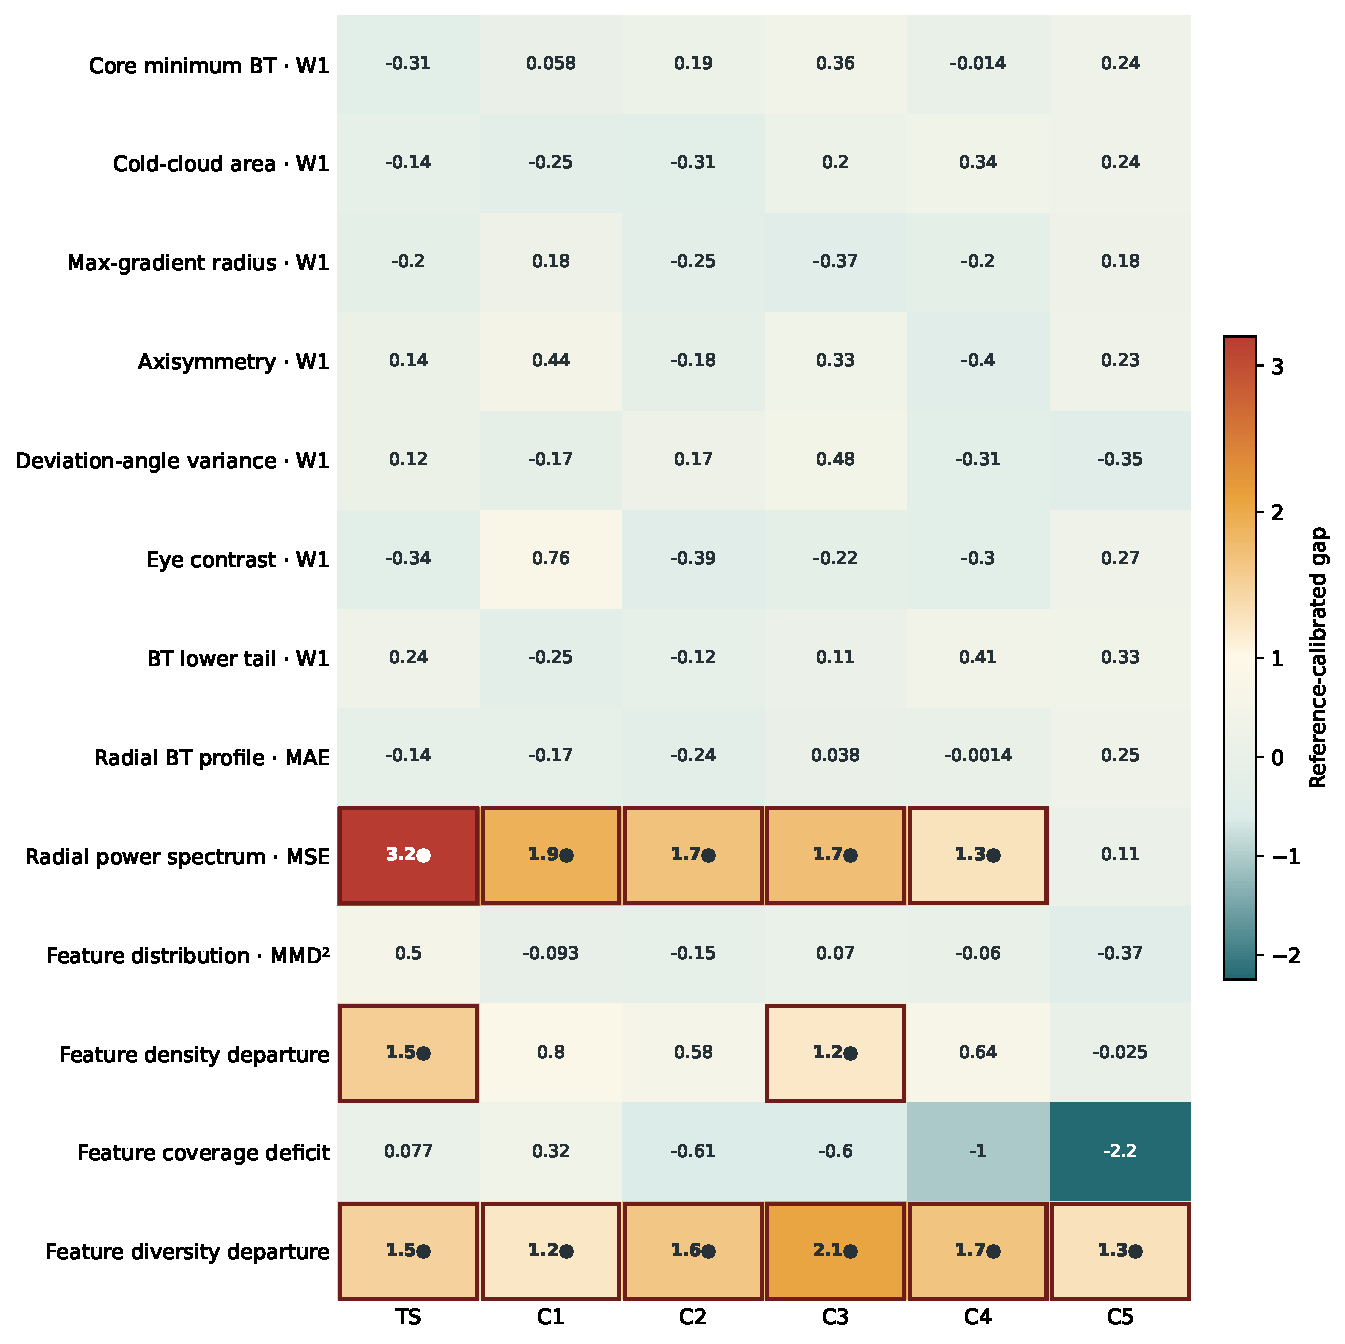
\includegraphics[width=16cm]{figS01.pdf}
\caption{Complete six-class by metric reference-gap matrix. The marker encodes the
empirical reference status for each independently interpreted comparison. The gap is a
presentation scale conditional on the archive and evaluation design, not physical
severity or an aggregate model score.}
\label{fig:smatrix}
\end{figure}

\clearpage
\tablecaption{Complete native-unit conditional results underlying the reference-gap
profile. The reference column reports the empirical real-reference median and 95th
percentile. Central ranges condition on the fixed generated bank and the available
held-out archive.}
\label{tab:snative}
\tablehead{
\hline
Class & Metric & Model discrepancy [central range] & Reference $q_{50}\rightarrow q_{95}$ & Gap & Status \\
\hline
}
\tabletail{\hline}
\begin{supertabular}{p{0.055\linewidth}p{0.23\linewidth}p{0.25\linewidth}p{0.22\linewidth}rr}
TS & Core minimum BT W1 & 0.893 [0.498, 1.72] K & 1.24 $\rightarrow$ 2.33 K & -0.31 & within \\
C1 & Core minimum BT W1 & 1.29 [0.58, 2.46] K & 1.22 $\rightarrow$ 2.44 K & 0.058 & within \\
C2 & Core minimum BT W1 & 1.45 [0.637, 2.45] K & 1.24 $\rightarrow$ 2.31 K & 0.19 & within \\
C3 & Core minimum BT W1 & 1.38 [0.705, 2.31] K & 1.04 $\rightarrow$ 2.01 K & 0.36 & within \\
C4 & Core minimum BT W1 & 0.975 [0.496, 1.72] K & 0.988 $\rightarrow$ 1.99 K & -0.014 & within \\
C5 & Core minimum BT W1 & 2.44 [1, 4.3] K & 1.99 $\rightarrow$ 3.87 K & 0.24 & within \\
TS & Cold-cloud area W1 & 1.82 [0.831, 4.56] \% & 2.23 $\rightarrow$ 5.16 \% & -0.14 & within \\
C1 & Cold-cloud area W1 & 2.08 [0.98, 4.94] \% & 3.03 $\rightarrow$ 6.85 \% & -0.25 & within \\
C2 & Cold-cloud area W1 & 2.29 [1.19, 4.64] \% & 3.31 $\rightarrow$ 6.62 \% & -0.31 & within \\
C3 & Cold-cloud area W1 & 3.9 [1.96, 7.08] \% & 3.13 $\rightarrow$ 6.93 \% & 0.2 & within \\
C4 & Cold-cloud area W1 & 4.22 [2.01, 7.1] \% & 2.96 $\rightarrow$ 6.69 \% & 0.34 & within \\
C5 & Cold-cloud area W1 & 5.39 [2.5, 9.51] \% & 4.41 $\rightarrow$ 8.45 \% & 0.24 & within \\
TS & Max-gradient radius W1 & 6.8 [3.64, 12.8] km & 8.45 $\rightarrow$ 16.8 km & -0.2 & within \\
C1 & Max-gradient radius W1 & 14.3 [5.66, 27] km & 12.1 $\rightarrow$ 24.3 km & 0.18 & within \\
C2 & Max-gradient radius W1 & 11.2 [5.39, 20.4] km & 14.6 $\rightarrow$ 28.1 km & -0.25 & within \\
C3 & Max-gradient radius W1 & 10.6 [5.47, 20.9] km & 17 $\rightarrow$ 34.3 km & -0.37 & within \\
C4 & Max-gradient radius W1 & 16.8 [7.8, 37] km & 22 $\rightarrow$ 48.3 km & -0.2 & within \\
C5 & Max-gradient radius W1 & 56.6 [19.9, 110] km & 44.8 $\rightarrow$ 109 km & 0.18 & within \\
TS & Axisymmetry W1 & 0.446 [0.238, 0.749] K & 0.394 $\rightarrow$ 0.773 K & 0.14 & within \\
C1 & Axisymmetry W1 & 0.654 [0.295, 1.09] K & 0.456 $\rightarrow$ 0.903 K & 0.44 & within \\
C2 & Axisymmetry W1 & 0.397 [0.227, 0.737] K & 0.471 $\rightarrow$ 0.887 K & -0.18 & within \\
C3 & Axisymmetry W1 & 0.577 [0.318, 0.864] K & 0.447 $\rightarrow$ 0.84 K & 0.33 & within \\
C4 & Axisymmetry W1 & 0.366 [0.221, 0.678] K & 0.562 $\rightarrow$ 1.06 K & -0.4 & within \\
C5 & Axisymmetry W1 & 0.943 [0.564, 1.62] K & 0.779 $\rightarrow$ 1.48 K & 0.23 & within \\
TS & Deviation-angle variance W1 & 31.7 [19.2, 54.7] deg$^2$ & 28.4 $\rightarrow$ 55.3 deg$^2$ & 0.12 & within \\
C1 & Deviation-angle variance W1 & 37 [22.4, 62.2] deg$^2$ & 44.4 $\rightarrow$ 87.2 deg$^2$ & -0.17 & within \\
C2 & Deviation-angle variance W1 & 65.2 [38.7, 98.1] deg$^2$ & 57 $\rightarrow$ 104 deg$^2$ & 0.17 & within \\
C3 & Deviation-angle variance W1 & 72 [50.3, 101] deg$^2$ & 48.3 $\rightarrow$ 97.8 deg$^2$ & 0.48 & within \\
C4 & Deviation-angle variance W1 & 48.1 [26.1, 86.7] deg$^2$ & 69.2 $\rightarrow$ 137 deg$^2$ & -0.31 & within \\
C5 & Deviation-angle variance W1 & 117 [61.4, 220] deg$^2$ & 182 $\rightarrow$ 365 deg$^2$ & -0.35 & within \\
TS & Eye contrast W1 & 0.456 [0.281, 0.756] K & 0.603 $\rightarrow$ 1.04 K & -0.34 & within \\
C1 & Eye contrast W1 & 1.18 [0.707, 1.76] K & 0.762 $\rightarrow$ 1.31 K & 0.76 & within \\
C2 & Eye contrast W1 & 0.799 [0.518, 1.32] K & 1.15 $\rightarrow$ 2.04 K & -0.39 & within \\
C3 & Eye contrast W1 & 0.982 [0.559, 1.83] K & 1.19 $\rightarrow$ 2.13 K & -0.22 & within \\
C4 & Eye contrast W1 & 1.23 [0.733, 2.77] K & 1.83 $\rightarrow$ 3.84 K & -0.3 & within \\
C5 & Eye contrast W1 & 5.52 [2.77, 9.47] K & 4.32 $\rightarrow$ 8.8 K & 0.27 & within \\
TS & BT lower-tail W1 & 1.46 [0.631, 2.71] K & 1.18 $\rightarrow$ 2.34 K & 0.24 & within \\
C1 & BT lower-tail W1 & 0.951 [0.546, 1.73] K & 1.28 $\rightarrow$ 2.6 K & -0.25 & within \\
C2 & BT lower-tail W1 & 1.06 [0.523, 2.1] K & 1.21 $\rightarrow$ 2.39 K & -0.12 & within \\
C3 & BT lower-tail W1 & 1.2 [0.718, 1.94] K & 1.08 $\rightarrow$ 2.14 K & 0.11 & within \\
C4 & BT lower-tail W1 & 1.45 [0.893, 2.08] K & 1.01 $\rightarrow$ 2.09 K & 0.41 & within \\
C5 & BT lower-tail W1 & 2.5 [1.22, 4.28] K & 1.9 $\rightarrow$ 3.73 K & 0.33 & within \\
TS & Radial BT profile MAE & 0.831 [0.189, 2.56] K & 1.09 $\rightarrow$ 2.96 K & -0.14 & within \\
C1 & Radial BT profile MAE & 1.02 [0.424, 2.44] K & 1.36 $\rightarrow$ 3.4 K & -0.17 & within \\
C2 & Radial BT profile MAE & 0.991 [0.376, 2.24] K & 1.44 $\rightarrow$ 3.33 K & -0.24 & within \\
C3 & Radial BT profile MAE & 1.39 [0.451, 3.15] K & 1.31 $\rightarrow$ 3.38 K & 0.038 & within \\
C4 & Radial BT profile MAE & 1.58 [0.445, 3.35] K & 1.59 $\rightarrow$ 3.72 K & -0.0014 & within \\
C5 & Radial BT profile MAE & 3.9 [1.41, 6.8] K & 2.98 $\rightarrow$ 6.61 K & 0.25 & within \\
TS & Radial power-spectrum MSE & 0.00228 [0.00162, 0.00321] dex$^2$ & 2.98e-04 $\rightarrow$ 9.16e-04 dex$^2$ & 3.2 & above \\
C1 & Radial power-spectrum MSE & 0.00248 [0.00167, 0.00367] dex$^2$ & 5.07e-04 $\rightarrow$ 0.00155 dex$^2$ & 1.9 & above \\
C2 & Radial power-spectrum MSE & 0.00271 [0.00174, 0.00411] dex$^2$ & 6.65e-04 $\rightarrow$ 0.00188 dex$^2$ & 1.7 & above \\
C3 & Radial power-spectrum MSE & 0.00375 [0.00239, 0.00569] dex$^2$ & 8.59e-04 $\rightarrow$ 0.00253 dex$^2$ & 1.7 & above \\
C4 & Radial power-spectrum MSE & 0.00445 [0.00281, 0.00659] dex$^2$ & 0.00127 $\rightarrow$ 0.00377 dex$^2$ & 1.3 & above \\
C5 & Radial power-spectrum MSE & 0.0057 [0.00297, 0.011] dex$^2$ & 0.00464 $\rightarrow$ 0.0141 dex$^2$ & 0.11 & within \\
TS & Feature MMD$^2$ & 0.00592 [0.00378, 0.00937] MMD$^2$ & 0.00457 $\rightarrow$ 0.00725 MMD$^2$ & 0.5 & within \\
C1 & Feature MMD$^2$ & 0.00558 [0.00363, 0.00859] MMD$^2$ & 0.0059 $\rightarrow$ 0.00934 MMD$^2$ & -0.093 & within \\
C2 & Feature MMD$^2$ & 0.00678 [0.00465, 0.0096] MMD$^2$ & 0.00738 $\rightarrow$ 0.0114 MMD$^2$ & -0.15 & within \\
C3 & Feature MMD$^2$ & 0.0091 [0.00644, 0.0129] MMD$^2$ & 0.00879 $\rightarrow$ 0.0132 MMD$^2$ & 0.07 & within \\
C4 & Feature MMD$^2$ & 0.0114 [0.00808, 0.016] MMD$^2$ & 0.0119 $\rightarrow$ 0.0186 MMD$^2$ & -0.06 & within \\
C5 & Feature MMD$^2$ & 0.0352 [0.024, 0.0541] MMD$^2$ & 0.0437 $\rightarrow$ 0.0668 MMD$^2$ & -0.37 & within \\
TS & Feature-density departure & 0.305 [0.187, 0.412] absolute density departure & 0.0922 $\rightarrow$ 0.231 absolute density departure & 1.5 & above \\
C1 & Feature-density departure & 0.304 [0.161, 0.427] absolute density departure & 0.179 $\rightarrow$ 0.336 absolute density departure & 0.8 & within \\
C2 & Feature-density departure & 0.352 [0.204, 0.48] absolute density departure & 0.242 $\rightarrow$ 0.43 absolute density departure & 0.58 & within \\
C3 & Feature-density departure & 0.545 [0.417, 0.65] absolute density departure & 0.309 $\rightarrow$ 0.506 absolute density departure & 1.2 & above \\
C4 & Feature-density departure & 0.538 [0.408, 0.644] absolute density departure & 0.434 $\rightarrow$ 0.598 absolute density departure & 0.64 & within \\
C5 & Feature-density departure & 0.904 [0.794, 0.988] absolute density departure & 0.906 $\rightarrow$ 0.984 absolute density departure & -0.025 & within \\
TS & Feature-coverage deficit & 0.0703 [0.0312, 0.117] fraction & 0.0664 $\rightarrow$ 0.117 fraction & 0.077 & within \\
C1 & Feature-coverage deficit & 0.18 [0.105, 0.262] fraction & 0.156 $\rightarrow$ 0.23 fraction & 0.32 & within \\
C2 & Feature-coverage deficit & 0.215 [0.129, 0.309] fraction & 0.27 $\rightarrow$ 0.359 fraction & -0.61 & within \\
C3 & Feature-coverage deficit & 0.305 [0.207, 0.402] fraction & 0.363 $\rightarrow$ 0.461 fraction & -0.6 & within \\
C4 & Feature-coverage deficit & 0.367 [0.262, 0.469] fraction & 0.473 $\rightarrow$ 0.574 fraction & -1 & within \\
C5 & Feature-coverage deficit & 0.883 [0.785, 0.969] fraction & 0.953 $\rightarrow$ 0.984 fraction & -2.2 & within \\
TS & Feature-diversity departure & 0.0584 [0.0295, 0.092] relative departure & 0.0154 $\rightarrow$ 0.0444 relative departure & 1.5 & above \\
C1 & Feature-diversity departure & 0.0578 [0.0257, 0.0929] relative departure & 0.0188 $\rightarrow$ 0.051 relative departure & 1.2 & above \\
C2 & Feature-diversity departure & 0.0757 [0.0405, 0.109] relative departure & 0.0194 $\rightarrow$ 0.054 relative departure & 1.6 & above \\
C3 & Feature-diversity departure & 0.102 [0.0663, 0.142] relative departure & 0.0204 $\rightarrow$ 0.0602 relative departure & 2.1 & above \\
C4 & Feature-diversity departure & 0.0871 [0.0519, 0.127] relative departure & 0.0208 $\rightarrow$ 0.0608 relative departure & 1.7 & above \\
C5 & Feature-diversity departure & 0.119 [0.0669, 0.191] relative departure & 0.0368 $\rightarrow$ 0.101 relative departure & 1.3 & above \\
\hline
\end{supertabular}

\clearpage

\begin{table}[t]
\caption{Unmatched as-provided global comparison. The generated bank contains equal
numbers from TS and Categories 1--5, whereas the held-out archive has its natural,
strongly imbalanced intensity mixture. These values therefore audit dataset
composition and are not conditional model-fidelity results.}
\label{tab:sglobal}
\centering
\begin{tabular}{lrrrr}
\hline
Physical quantity & Model & Reference $q_{95}$ & Gap & Status \\
\hline
Core minimum BT & 2.29 K & 1.85 K & 1.5 & above \\
Cold-cloud area & 13.2 \% & 4.45 \% & 4.4 & above \\
Max-gradient radius & 15.2 km & 12.2 km & 1.5 & above \\
Axisymmetry & 2.57 K & 0.663 K & 6.3 & above \\
Deviation-angle variance & 140 deg$^2$ & 48 deg$^2$ & 4.6 & above \\
Eye contrast & 3.2 K & 0.82 K & 7.7 & above \\
BT lower tail & 2.89 K & 1.86 K & 2 & above \\
\hline
\end{tabular}

\end{table}

\section{Metric-specific controls}
\label{sec:scontrols}

Controls were constructed exclusively from reserved training storms. Each curve
reports the response over all declared severities rather than reducing the evidence
to a single label. A response can be monotone while remaining below the empirical
reference range; invariance controls have the opposite expectation.

\begin{figure}[t]
\centering
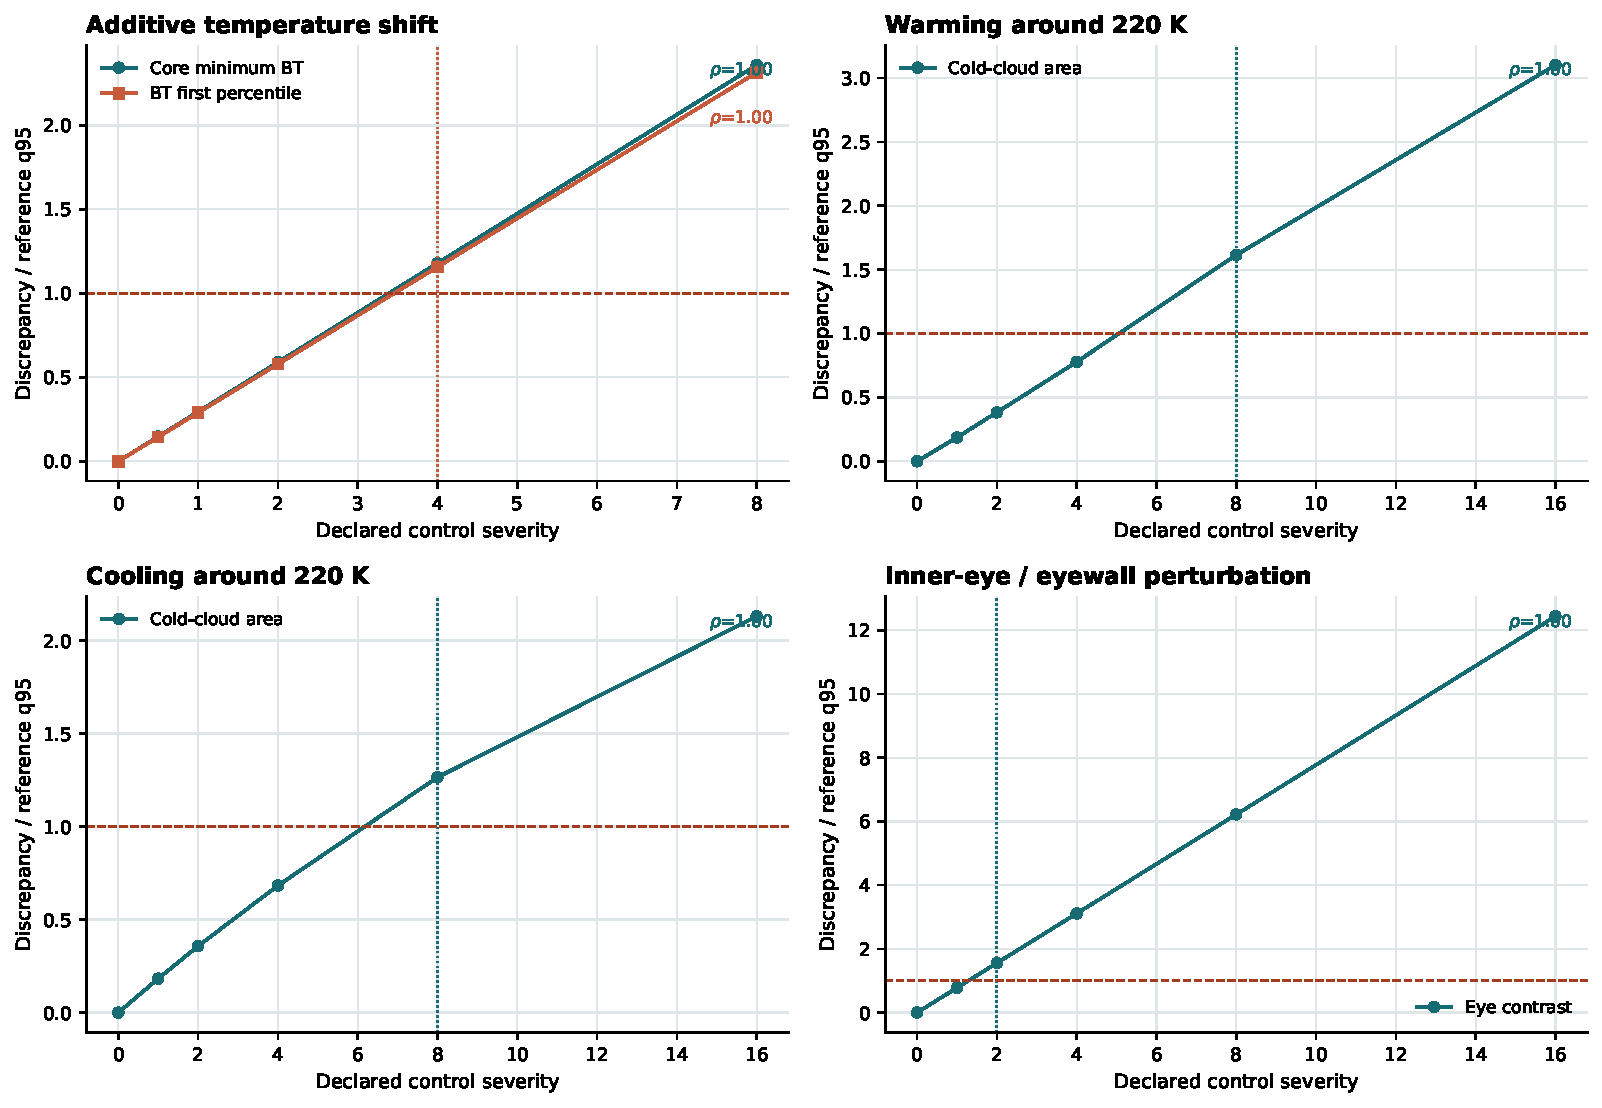
\includegraphics[width=16cm]{figS20.pdf}
\caption{Controls for the scalar physical quantities. Curves show discrepancy
relative to the empirical real-reference 95th-percentile marker at every declared
severity. Dotted vertical lines mark the first crossing where one occurs, and
\(\rho\) is Spearman's severity-response coefficient.}
\label{fig:sphysicalcontrols}
\end{figure}

\begin{figure}[t]
\centering
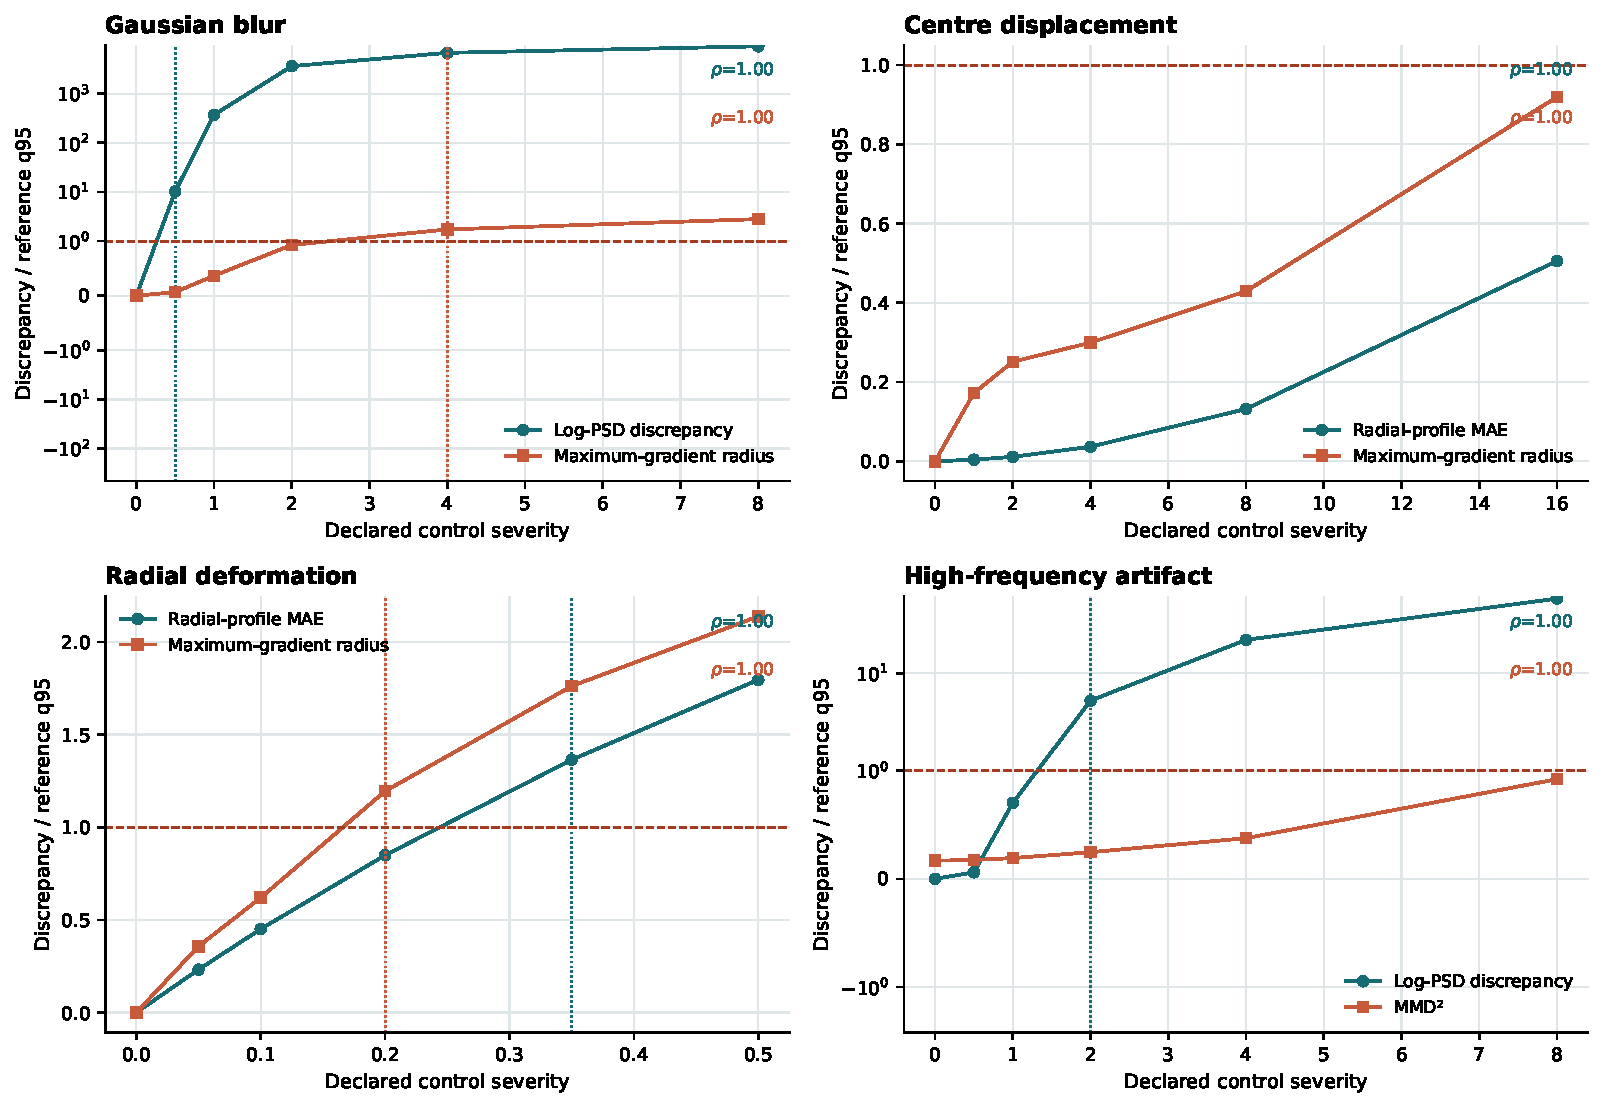
\includegraphics[width=16cm]{figS21.pdf}
\caption{Controls for storm geometry and spatial structure. Blur, centre
displacement, radial deformation, and a high-frequency artifact target different
spatial diagnostics rather than serving as interchangeable generic corruptions.}
\label{fig:sspatialcontrols}
\end{figure}

\begin{figure}[t]
\centering
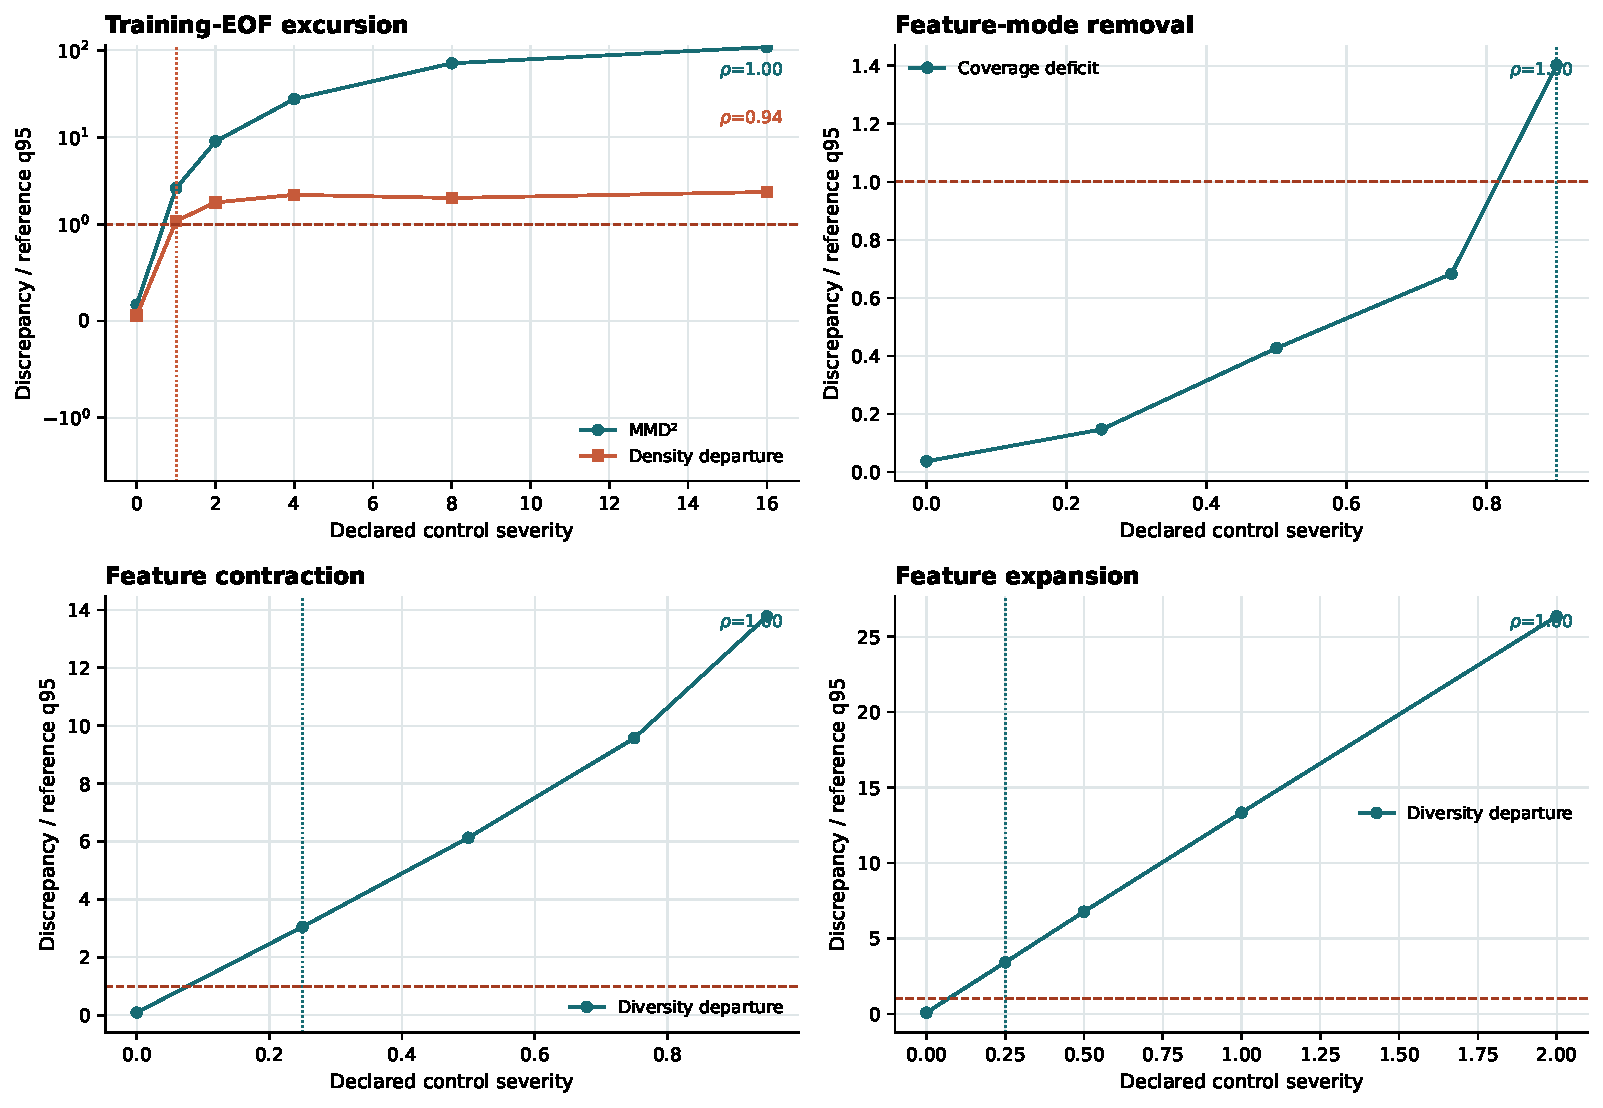
\includegraphics[width=16cm]{figS22.pdf}
\caption{Feature-space controls in the exact training-fitted representation used
by the reported TC metrics. A training-EOF excursion targets MMD\({}^2\) and
density, feature-mode removal targets coverage, and contraction and expansion
target the two directions of diversity departure.}
\label{fig:sfeaturecontrols}
\end{figure}

\begin{figure}[t]
\centering
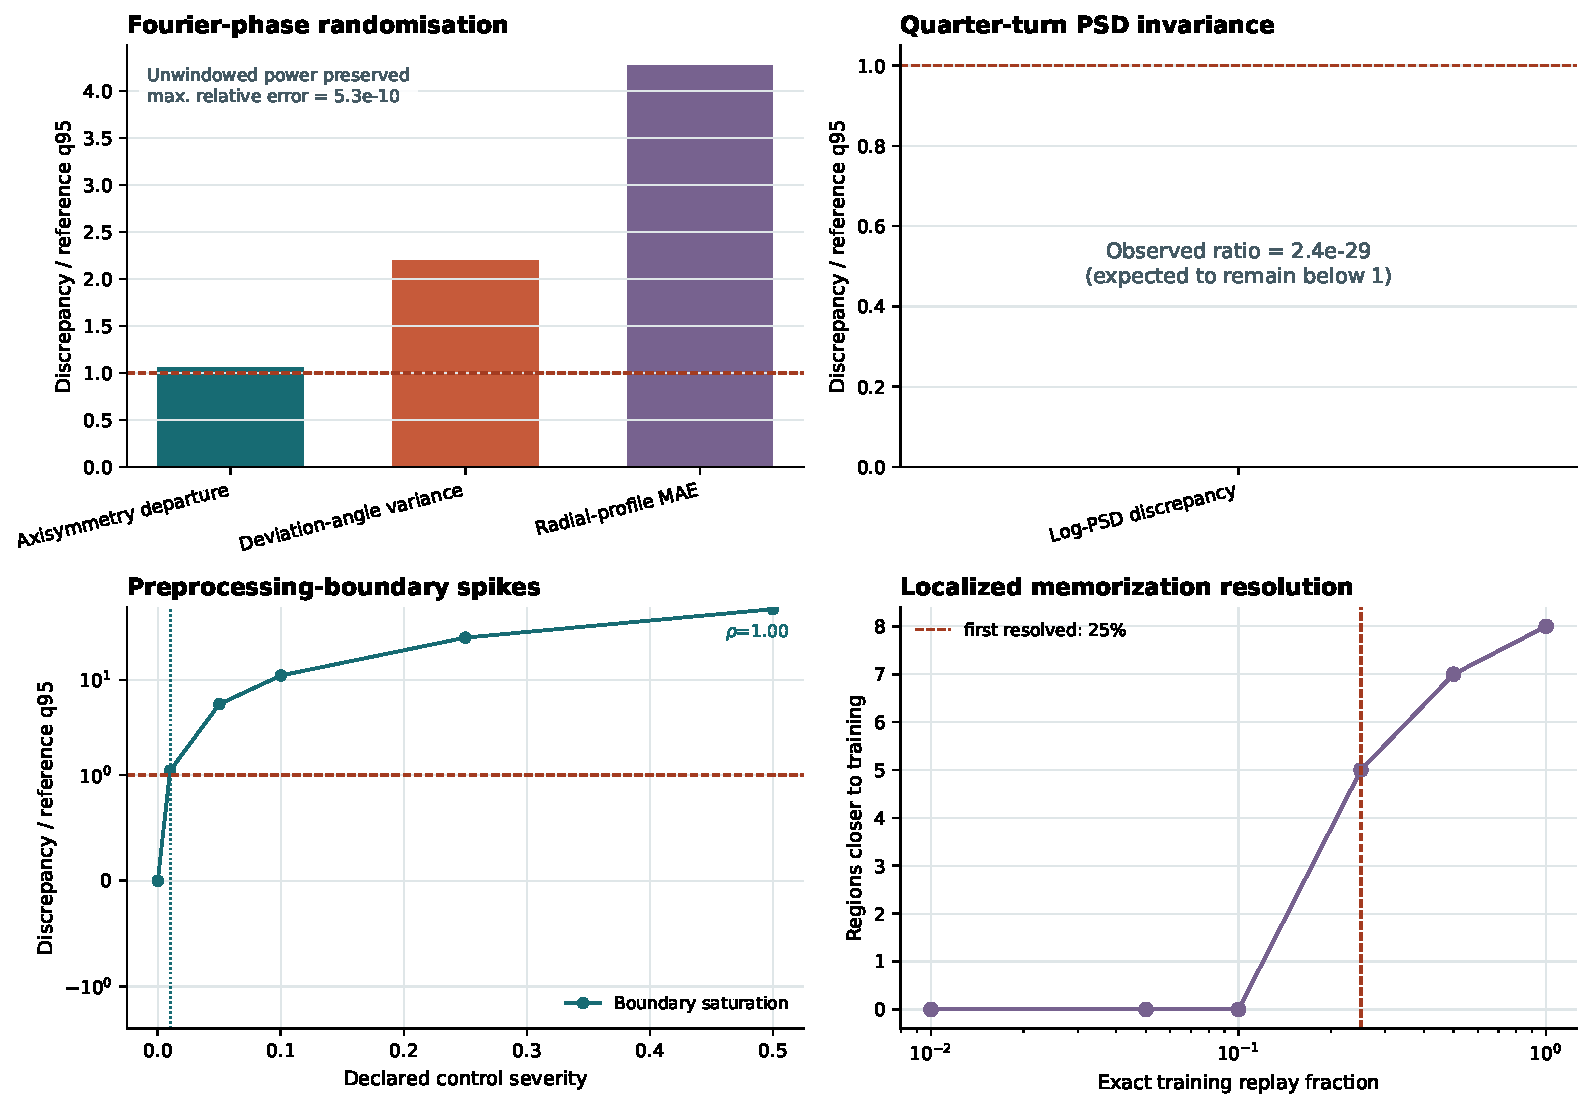
\includegraphics[width=16cm]{figS23.pdf}
\caption{Invariance and resolution controls. Fourier-phase randomisation disrupts
registered spatial-organisation diagnostics while preserving each field's
unwindowed Fourier magnitude; a quarter-turn leaves the radial Hann-windowed PSD
unchanged. Boundary spikes control preprocessing saturation, and the copied-fraction
curve records the smallest exact-replay mixture resolved by the localized
memorization audit.}
\label{fig:sinvariancecontrols}
\end{figure}

\section{All-class spatial curves}
\label{sec:scurves}

\begin{figure}[t]
\centering
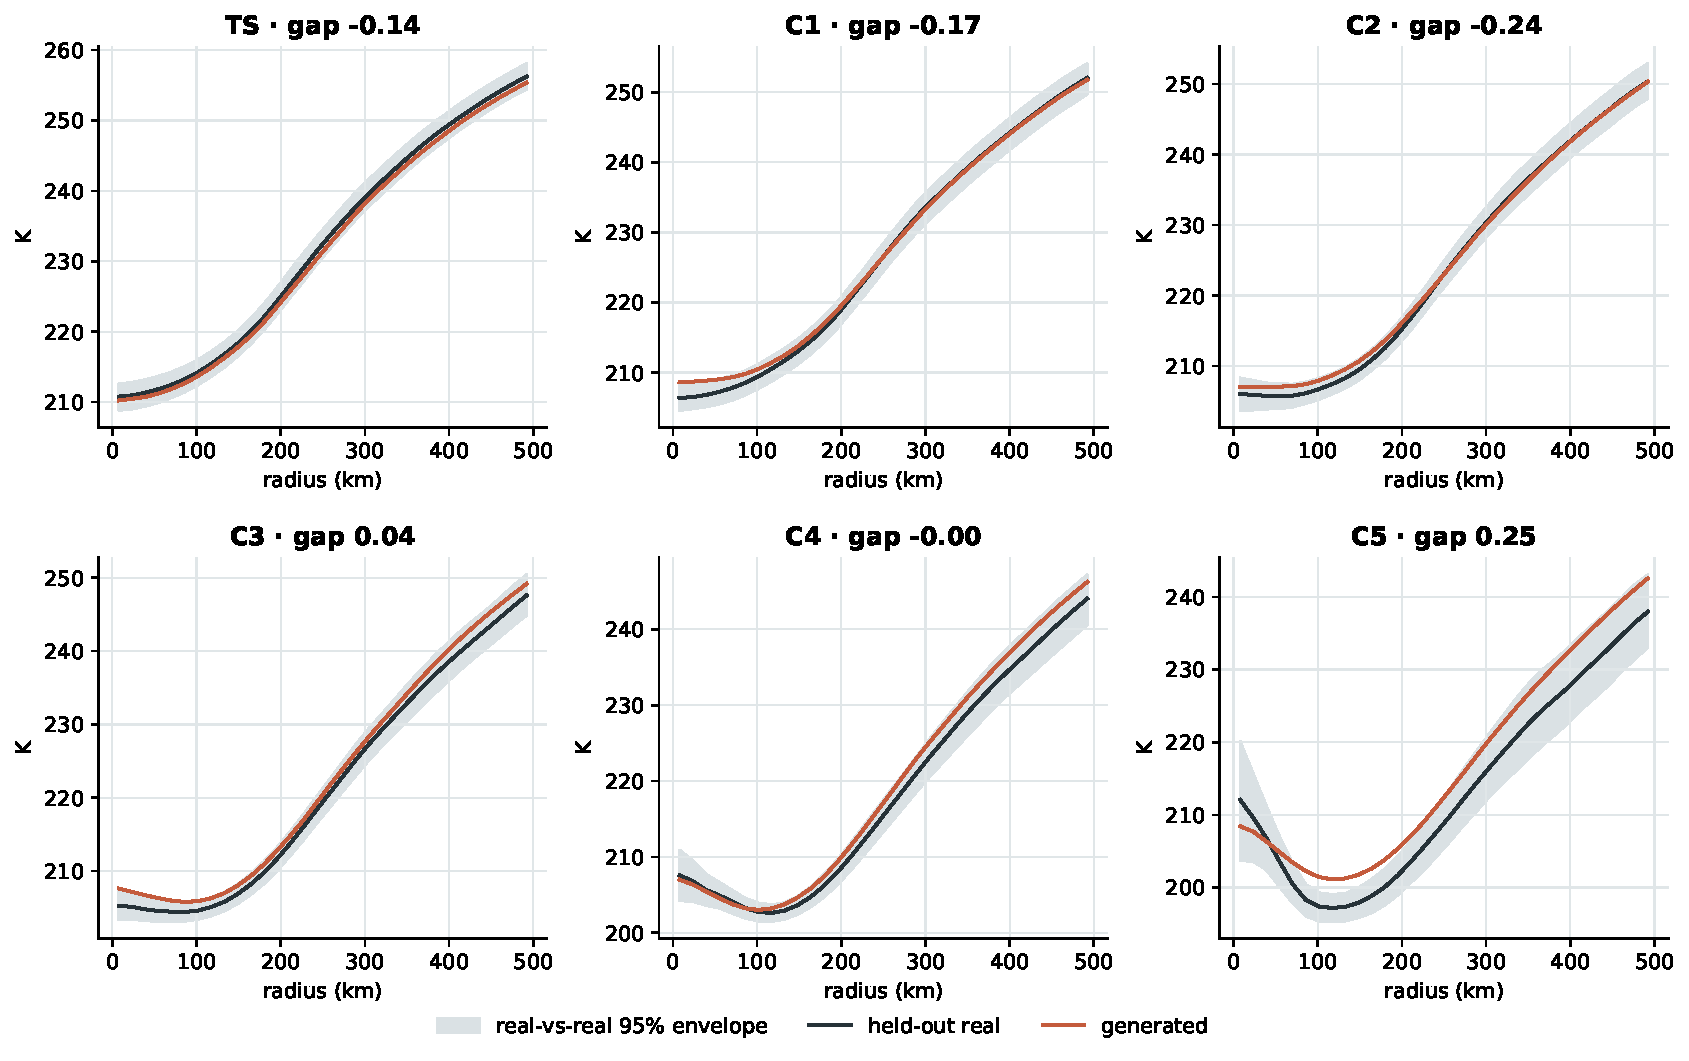
\includegraphics[width=16cm]{figS03.pdf}
\caption{Radial brightness-temperature profiles for held-out real and generated
fields in all six native intensity classes. Shading shows variation between admissible
real subsets at each radius; reference status is assigned from the scalar discrepancy
between complete curves.}
\label{fig:sprofiles}
\end{figure}

\begin{figure}[t]
\centering
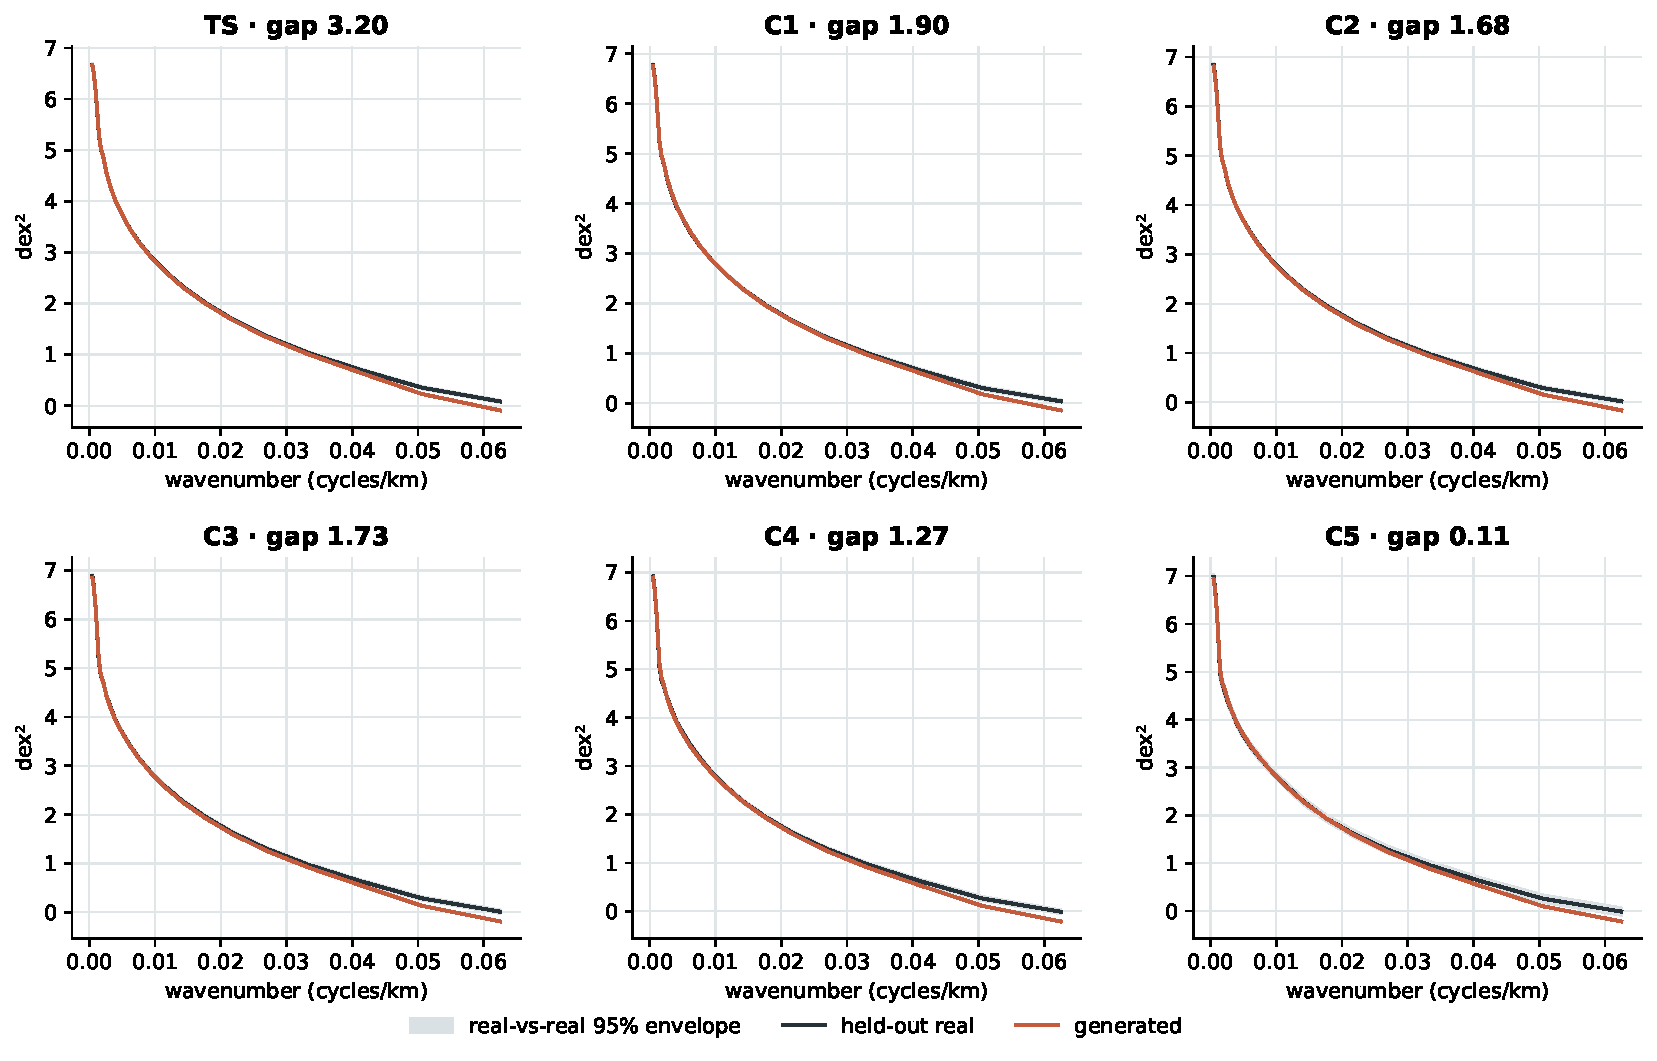
\includegraphics[width=16cm]{figS04.pdf}
\caption{Radial log-power curves for all six native intensity classes after
per-field mean removal, a separable Hann window, window-energy normalization, and
physical-wavenumber binning. The scalar discrepancy is mean squared log-power
difference in dex\({}^2\).}
\label{fig:spsd}
\end{figure}

\section{All-class physical distributions}
\label{sec:sfunctionals}

Figures~\ref{fig:sminbt}--\ref{fig:sp01} provide the class-resolved distributions
behind the seven scalar Wasserstein distances.

\begin{figure}[t]
\centering
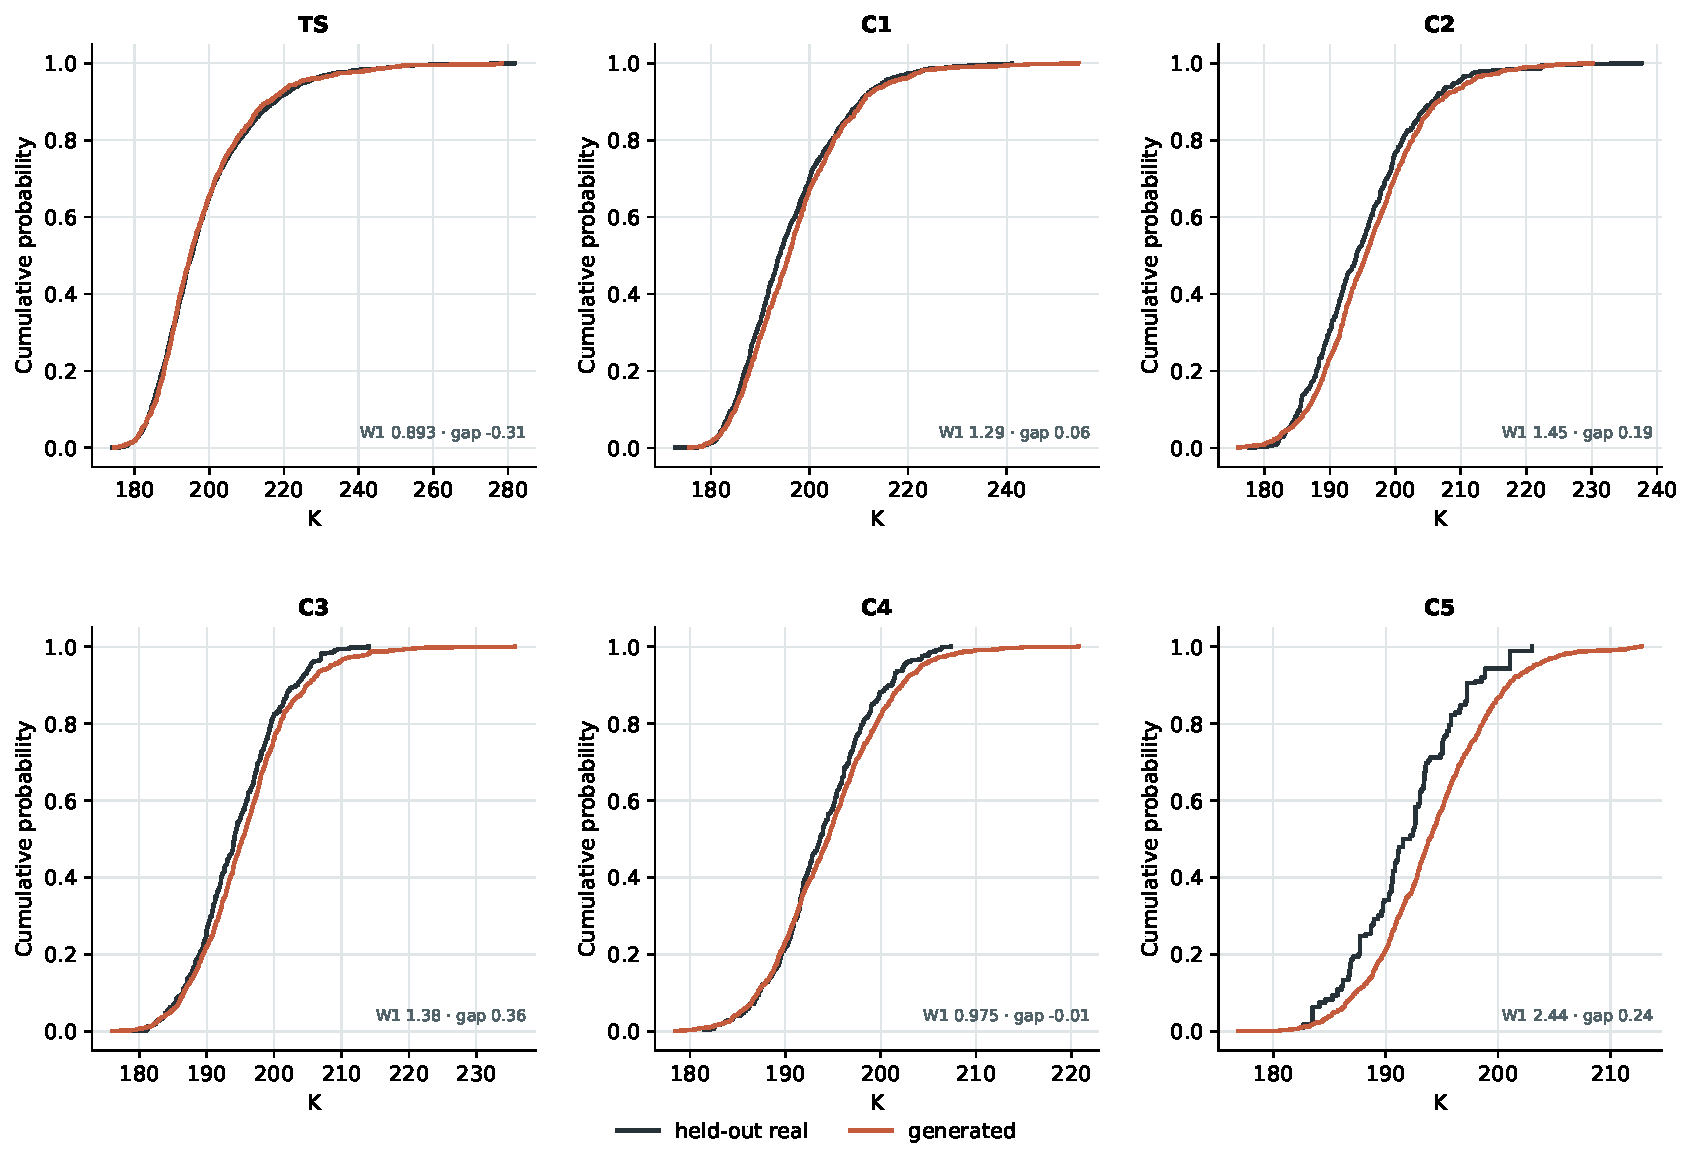
\includegraphics[width=16cm]{figS13.pdf}
\caption{Minimum core brightness temperature within 100\,km.}
\label{fig:sminbt}
\end{figure}

\begin{figure}[t]
\centering
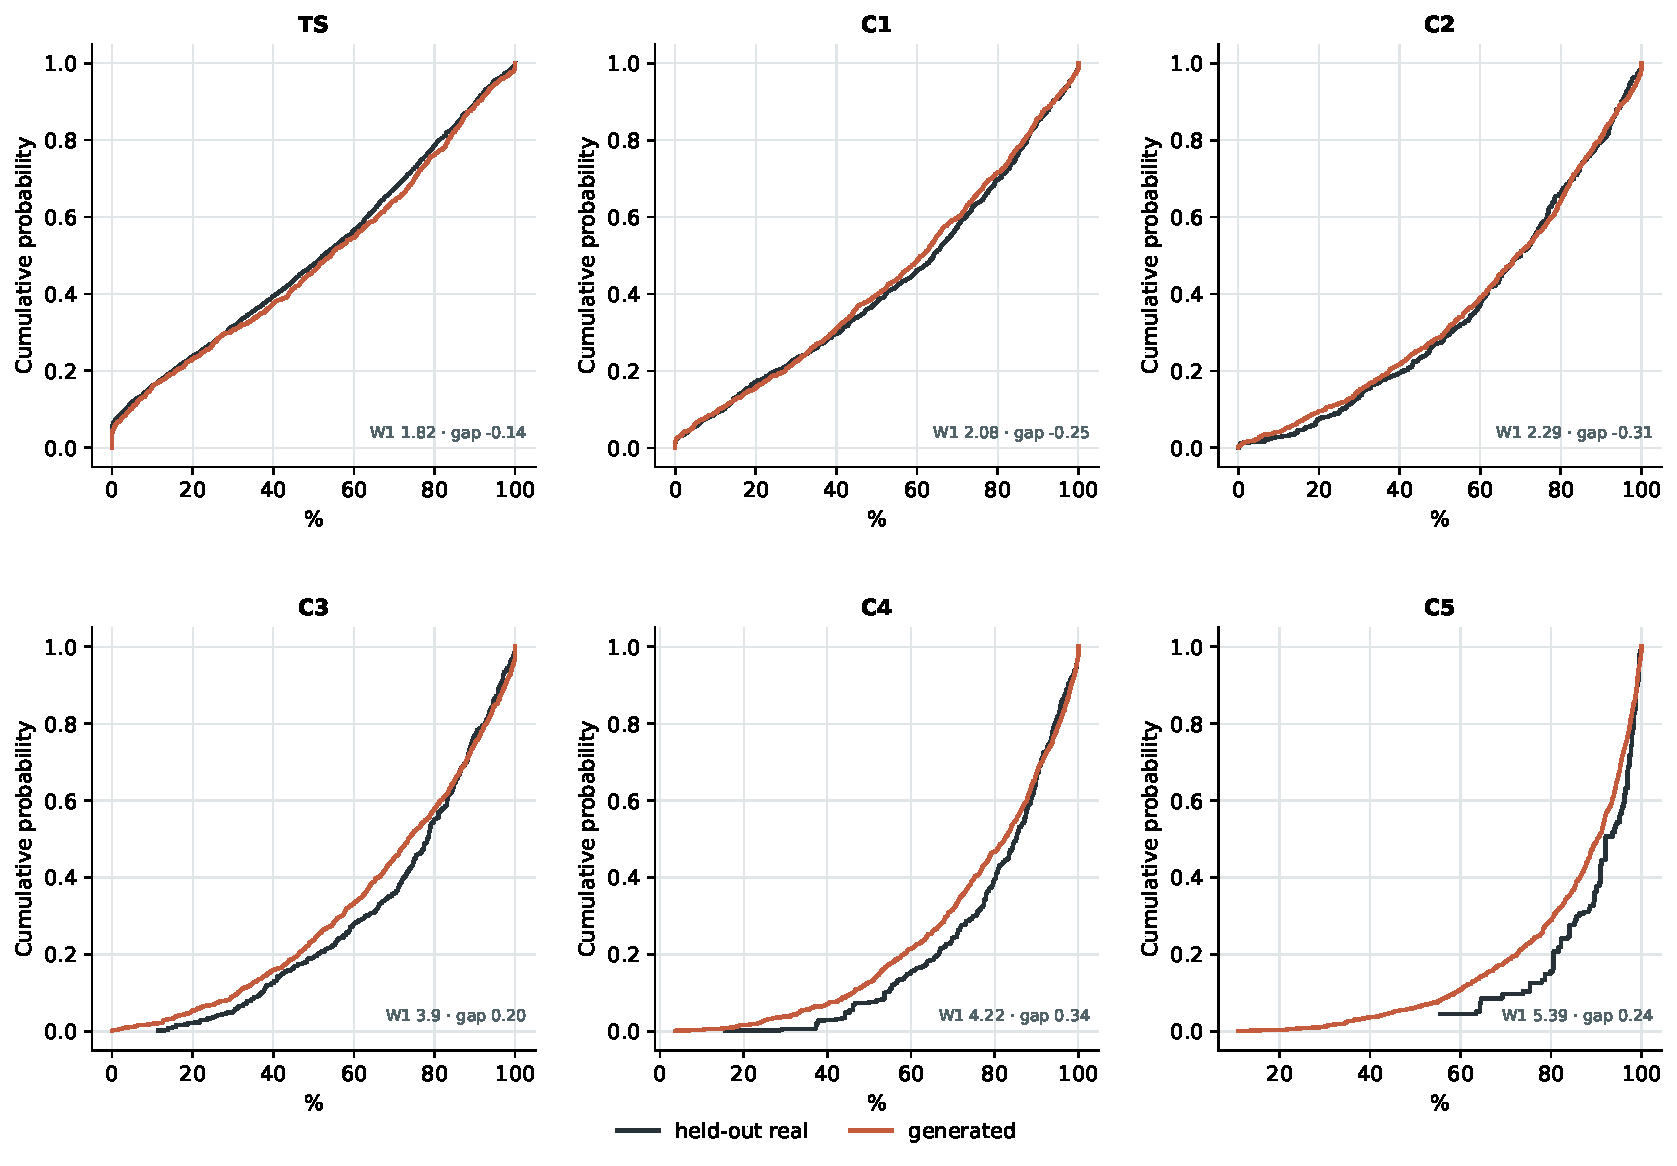
\includegraphics[width=16cm]{figS14.pdf}
\caption{Cold-cloud area below 220\,K within 300\,km.}
\label{fig:scold}
\end{figure}

\begin{figure}[t]
\centering
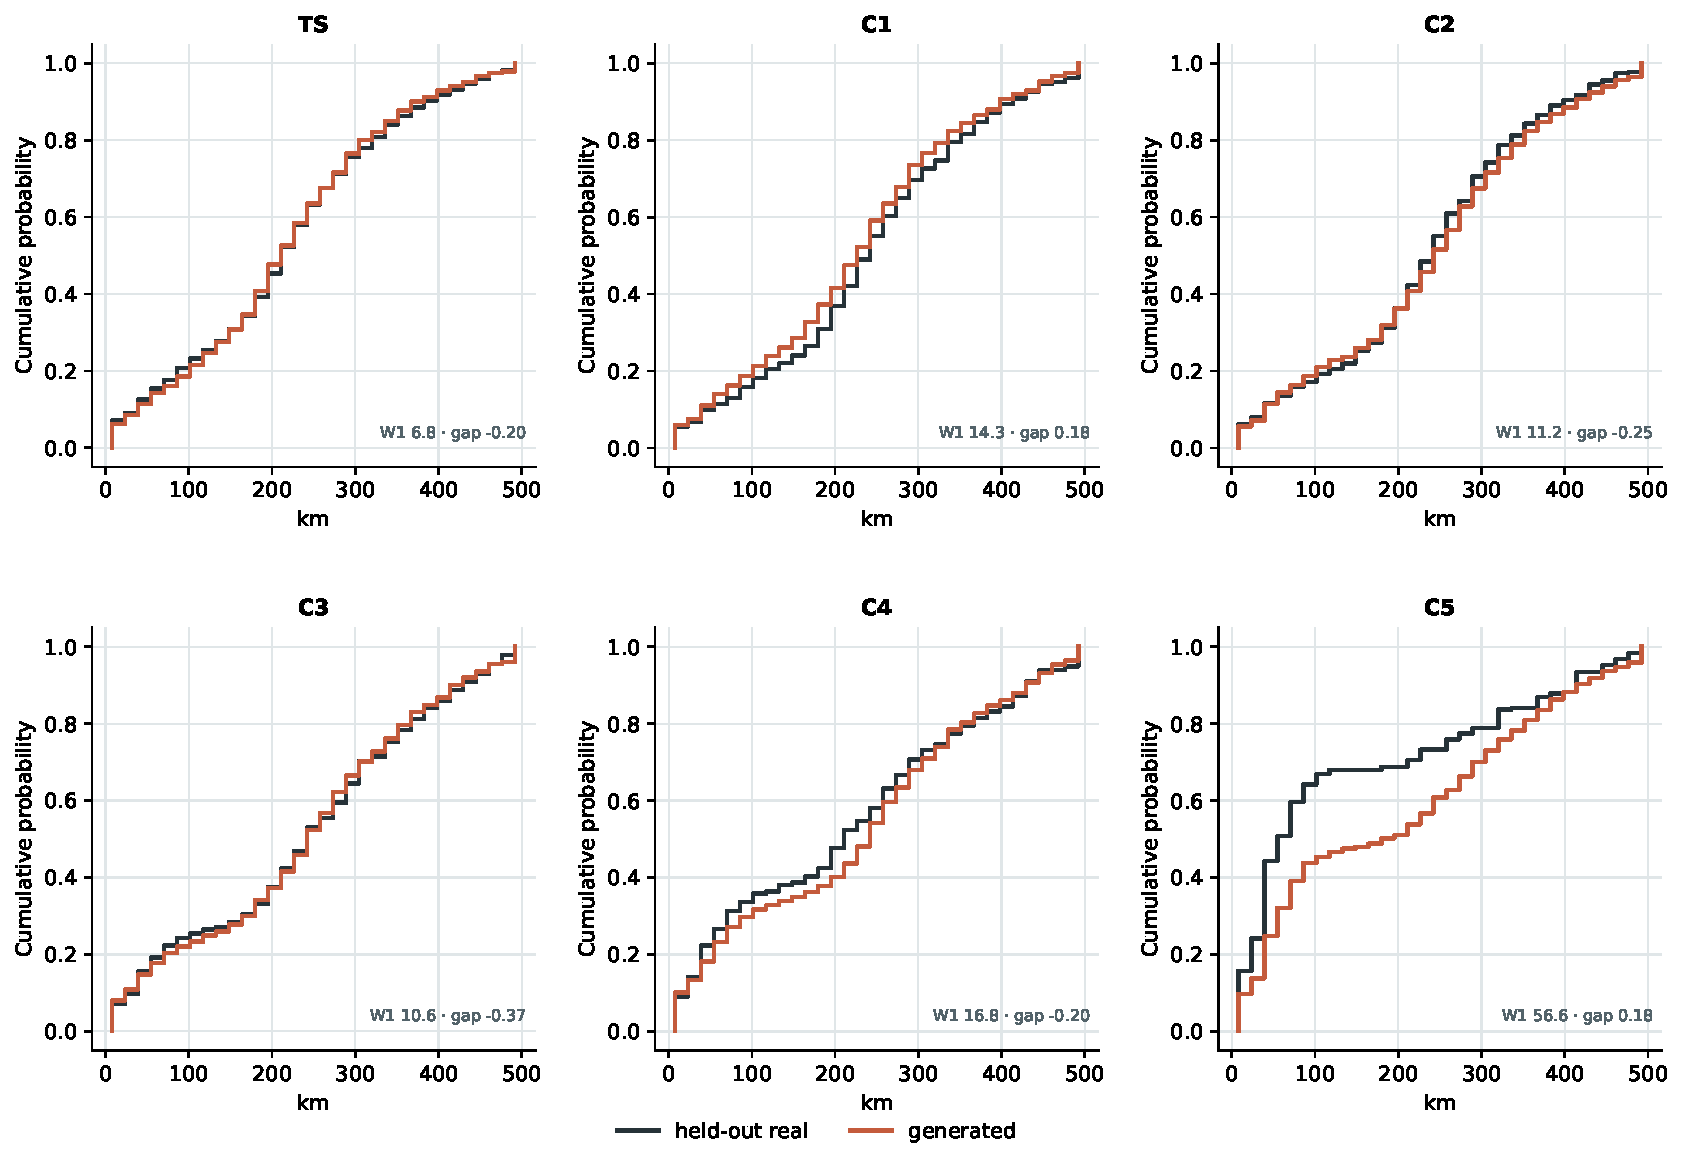
\includegraphics[width=16cm]{figS15.pdf}
\caption{Radius of the largest absolute radial-mean brightness-temperature
gradient.}
\label{fig:sradius}
\end{figure}

\begin{figure}[t]
\centering
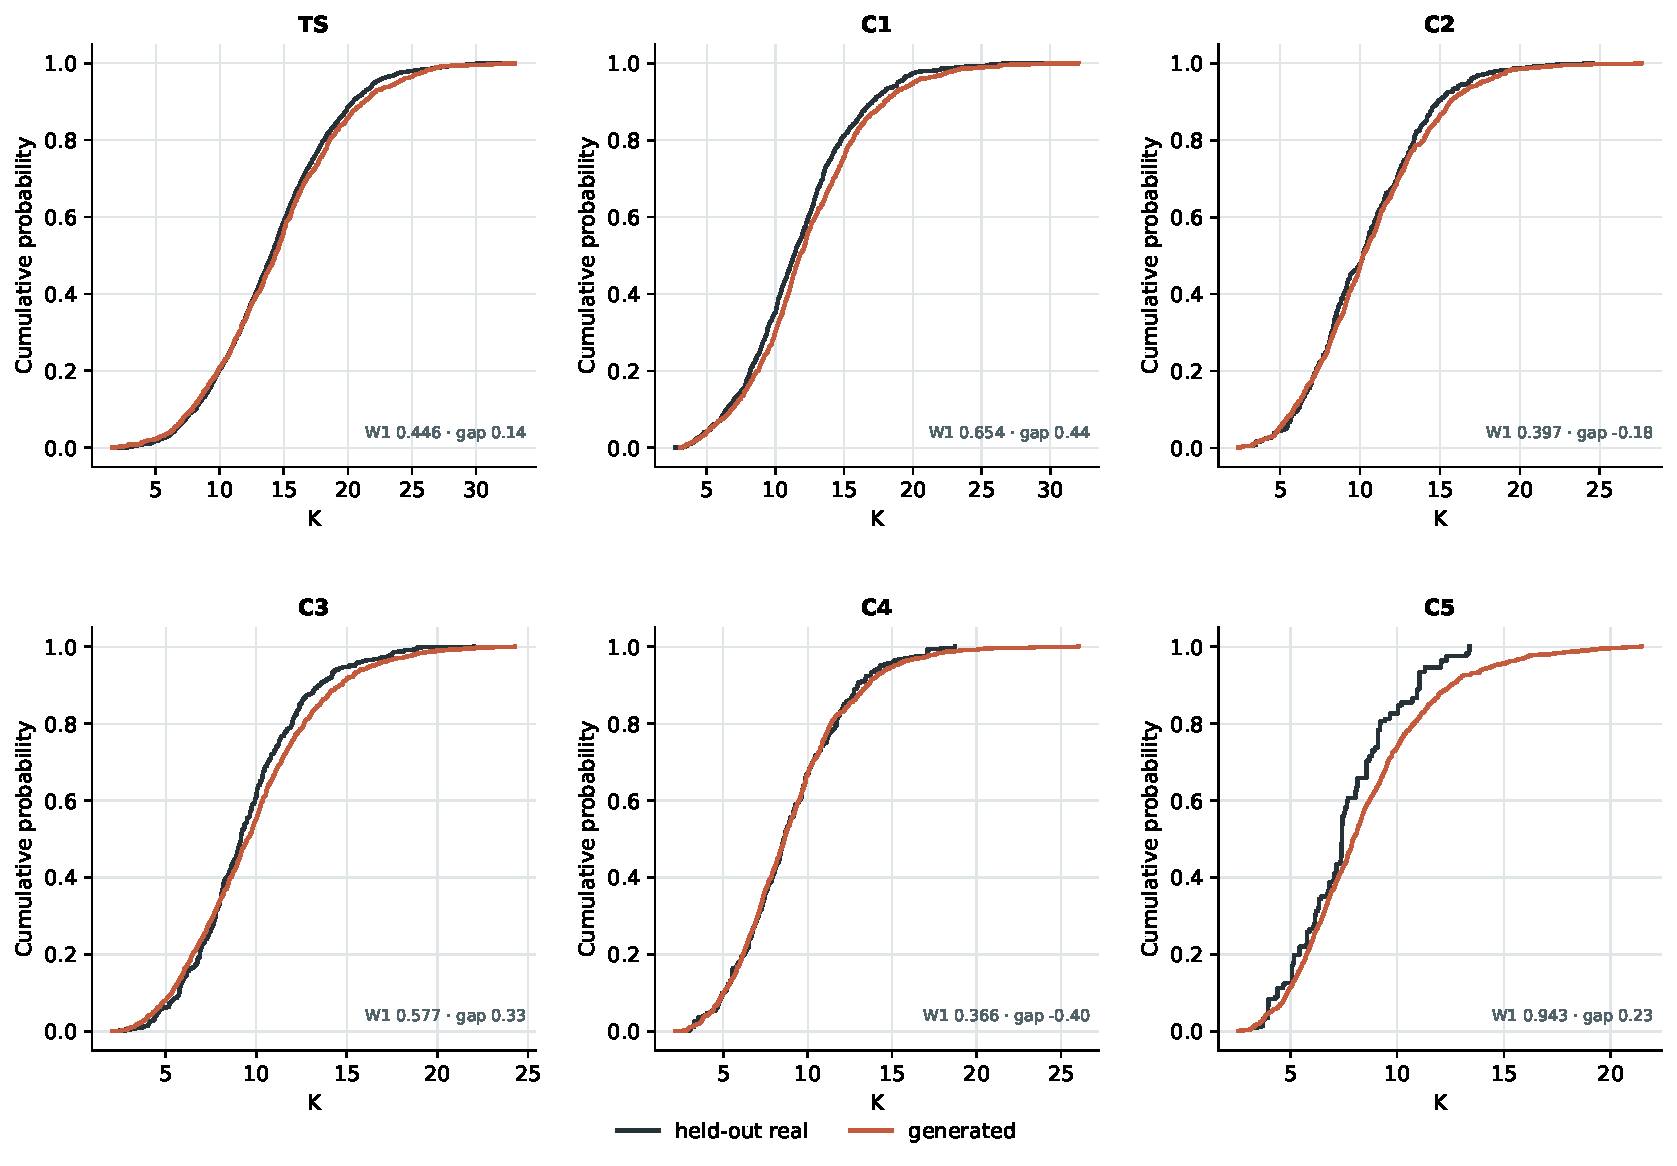
\includegraphics[width=16cm]{figS16.pdf}
\caption{Root-mean-square azimuthal brightness-temperature departure within
300\,km.}
\label{fig:saxisym}
\end{figure}

\begin{figure}[t]
\centering
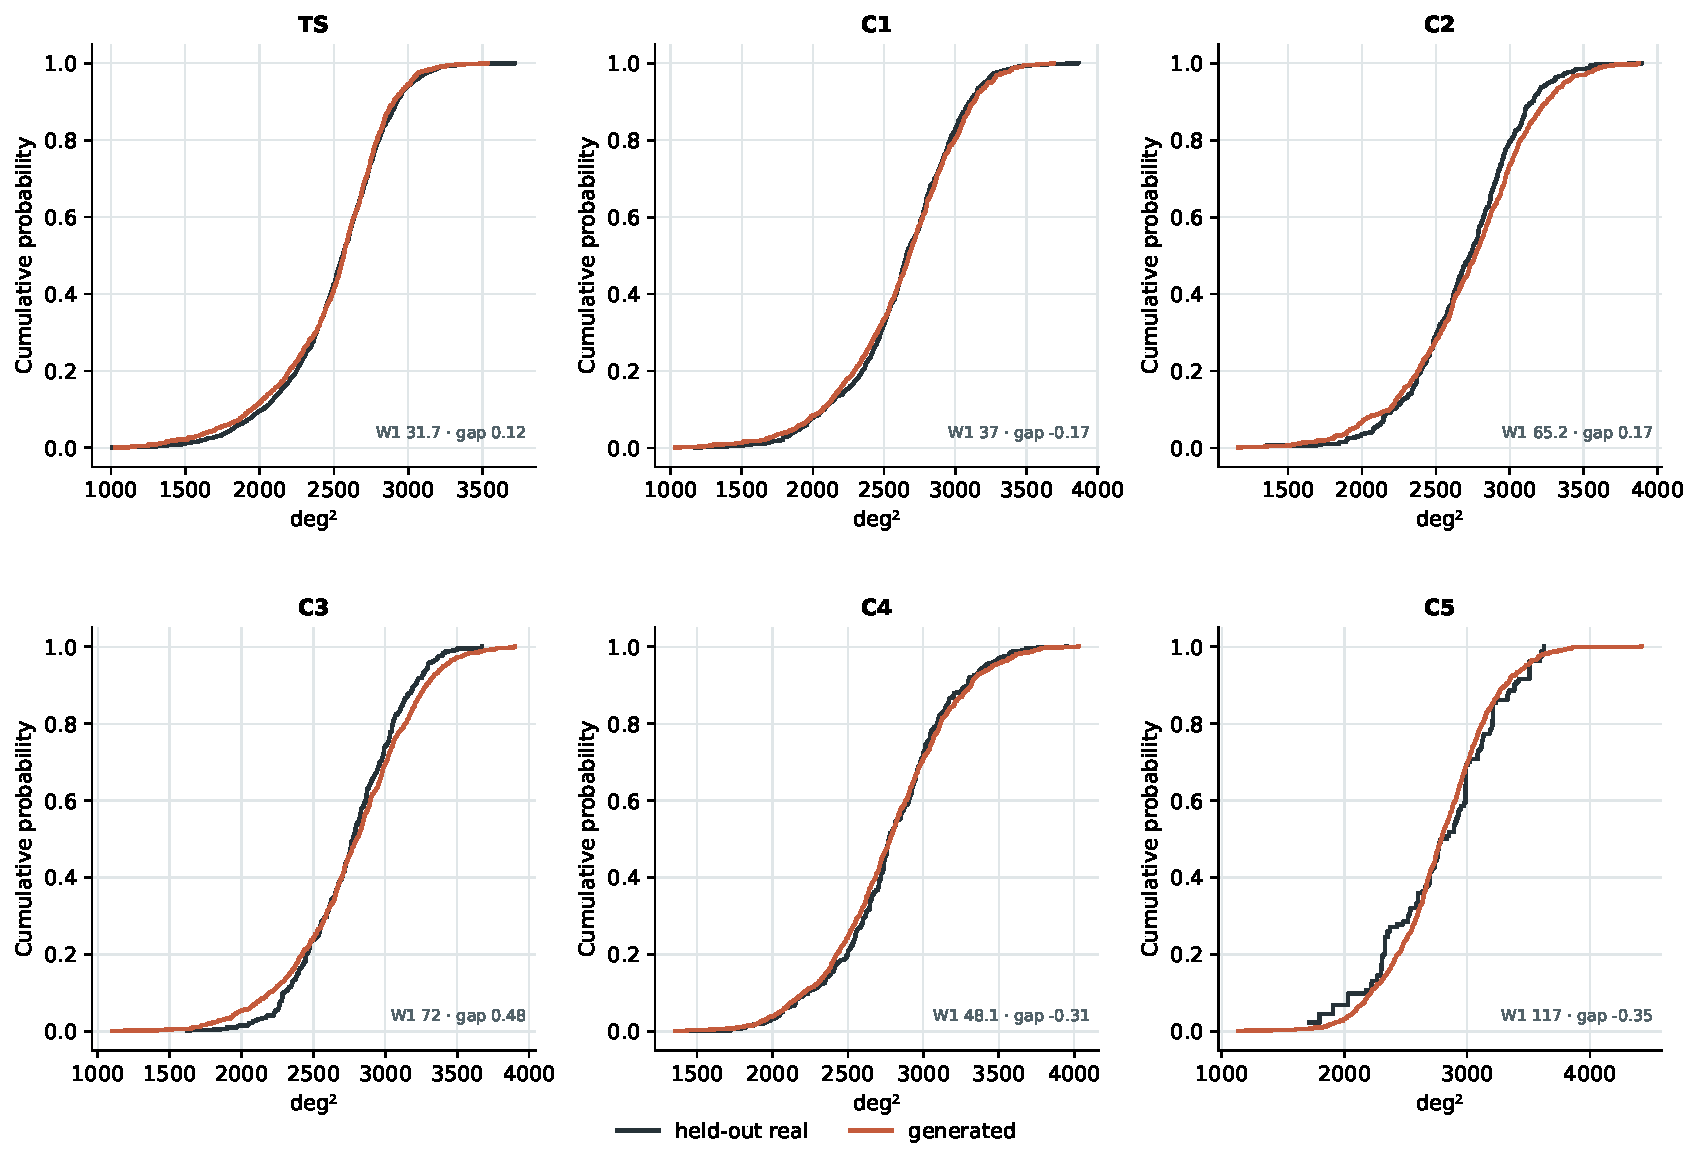
\includegraphics[width=16cm]{figS17.pdf}
\caption{Variance of the infrared-gradient deviation angle within 300\,km.}
\label{fig:sdav}
\end{figure}

\begin{figure}[t]
\centering
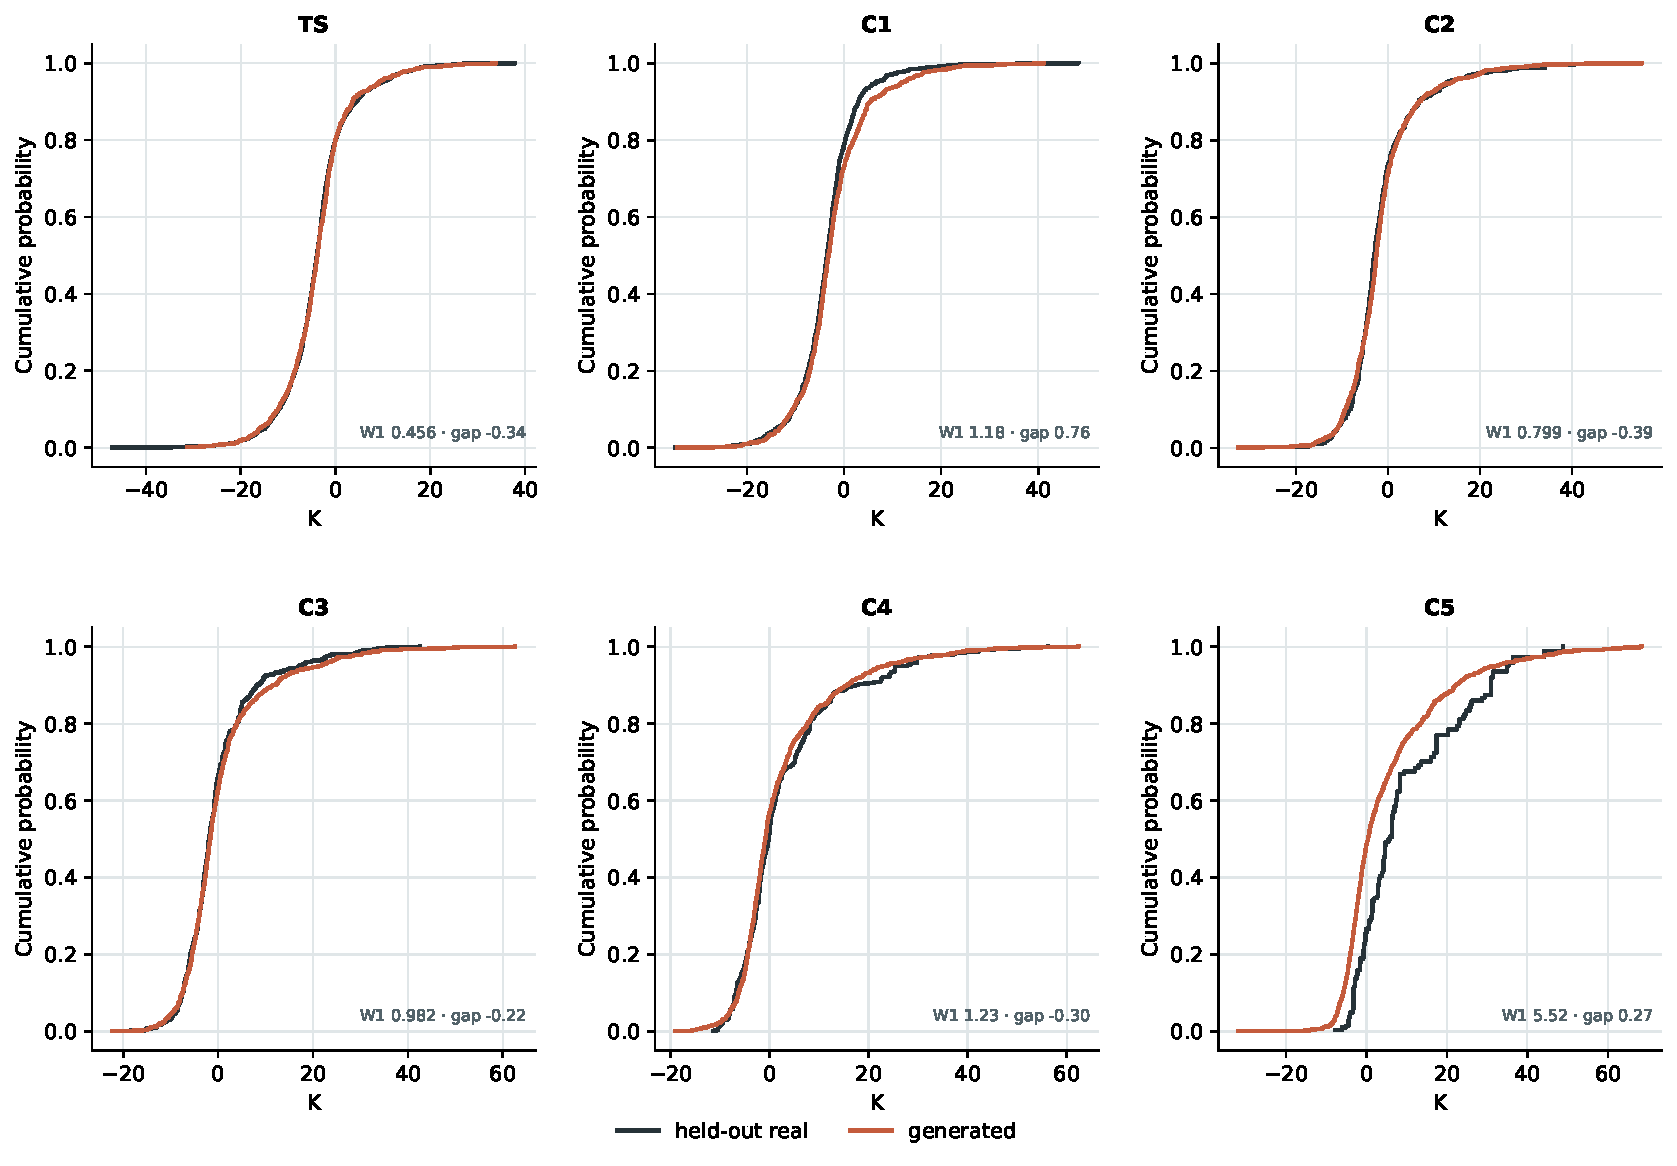
\includegraphics[width=16cm]{figS18.pdf}
\caption{Eye-to-eyewall brightness-temperature contrast.}
\label{fig:seye}
\end{figure}

\begin{figure}[t]
\centering
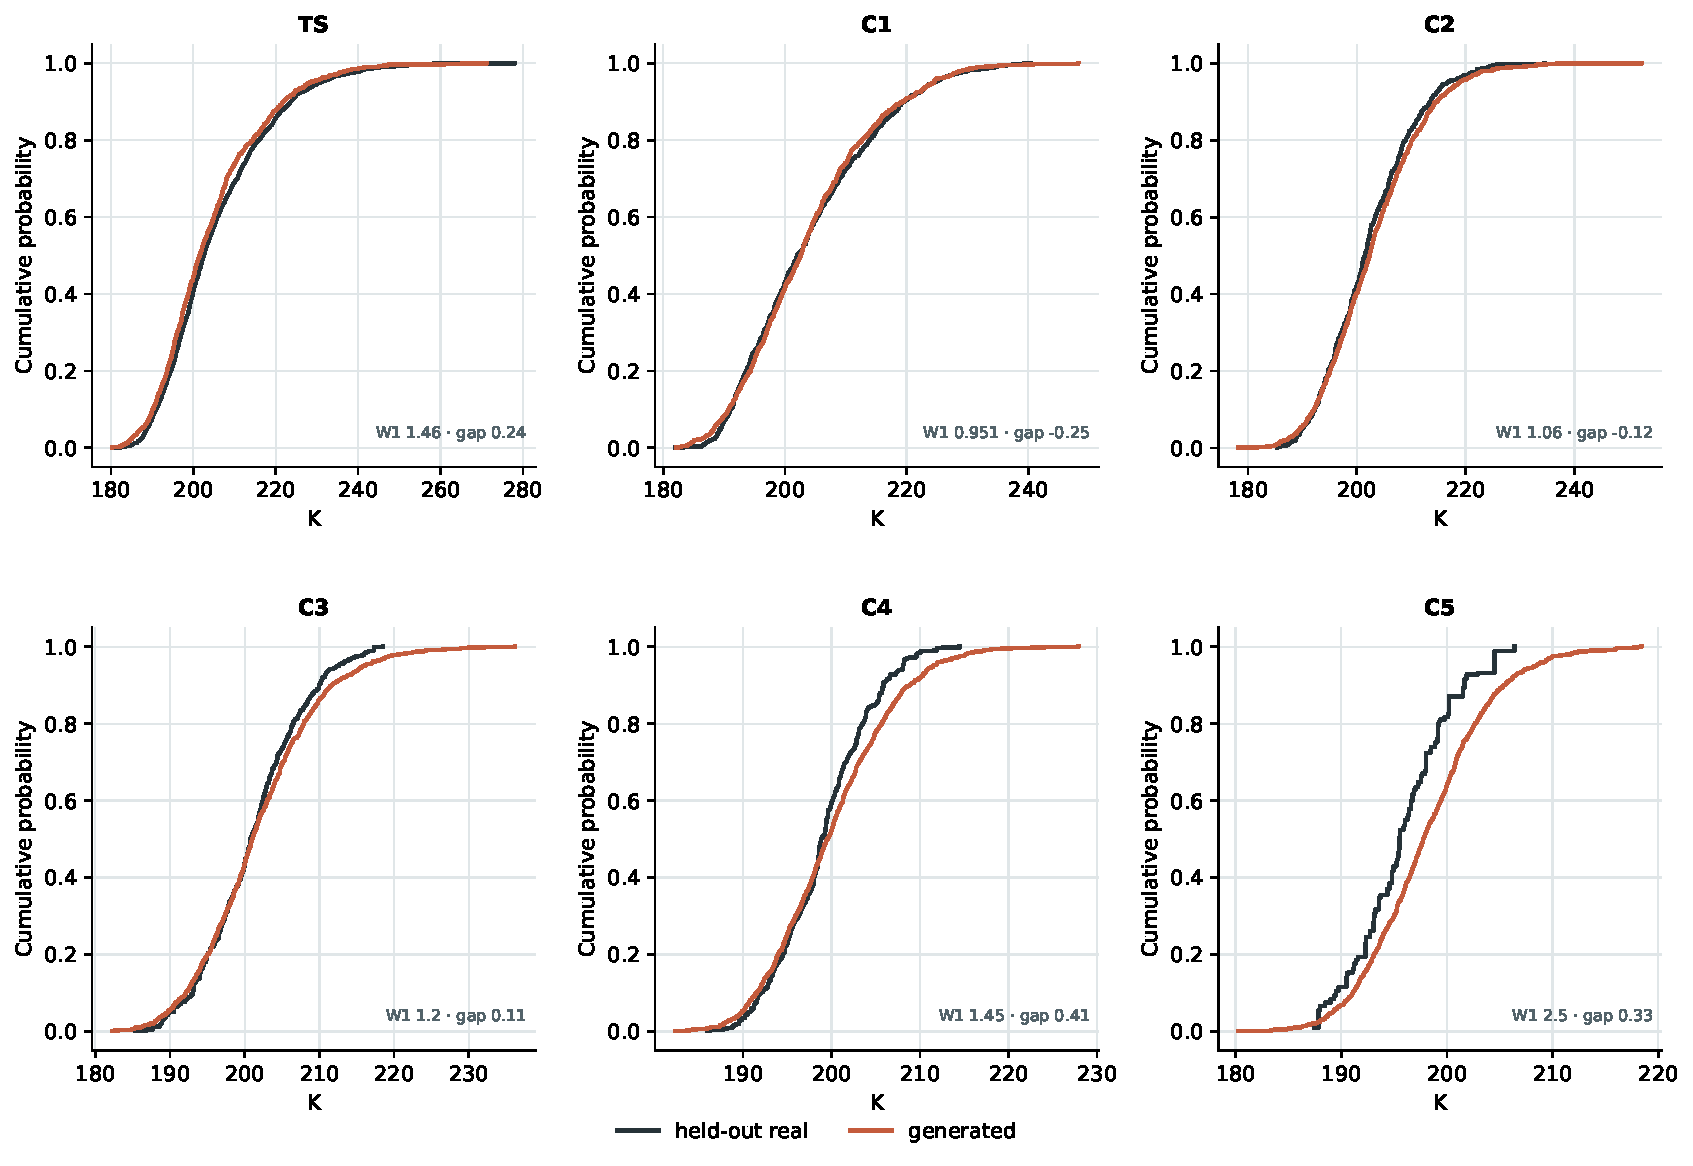
\includegraphics[width=16cm]{figS19.pdf}
\caption{Per-field first percentile of brightness temperature.}
\label{fig:sp01}
\end{figure}

\section{Feature, dependence, memorization, and preprocessing audits}
\label{sec:ssafeguards}

\begin{figure}[t]
\centering
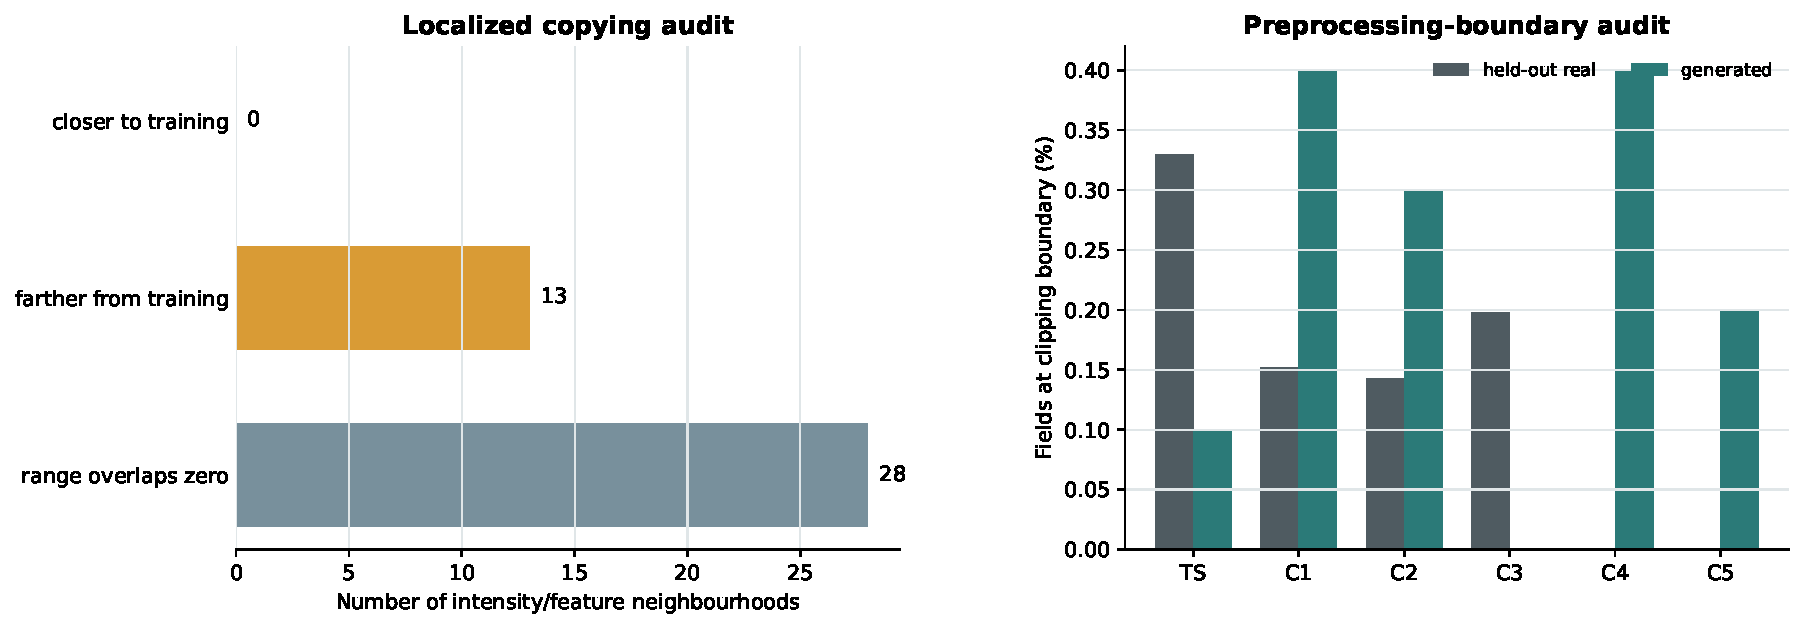
\includegraphics[width=16cm]{figS05.pdf}
\caption{Compact training-similarity and preprocessing-saturation audit. Similarity
is evaluated within supported intensity and training-fitted feature
neighbourhoods. Saturation refers to the fixed preprocessing bounds, not a universal
physical-admissibility criterion.}
\label{fig:ssafeguards}
\end{figure}

\begin{figure}[t]
\centering
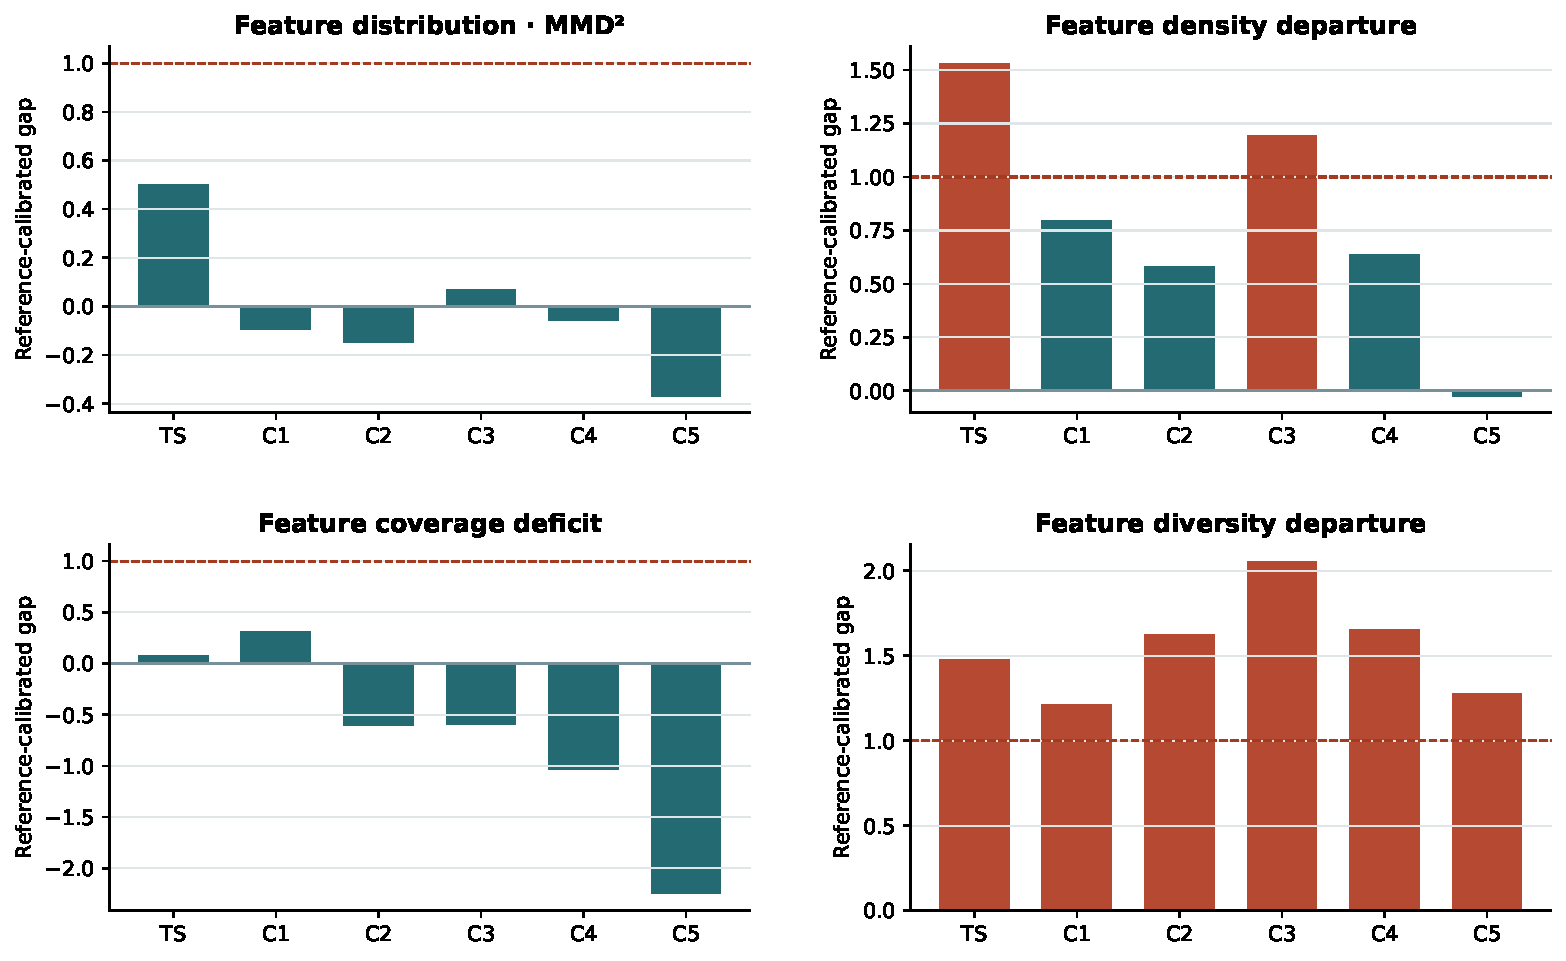
\includegraphics[width=16cm]{figS09.pdf}
\caption{Feature-space MMD\({}^2\), density, coverage, and diversity diagnostics
with direction and empirical reference context.}
\label{fig:sfeatures}
\end{figure}

\begin{figure}[t]
\centering
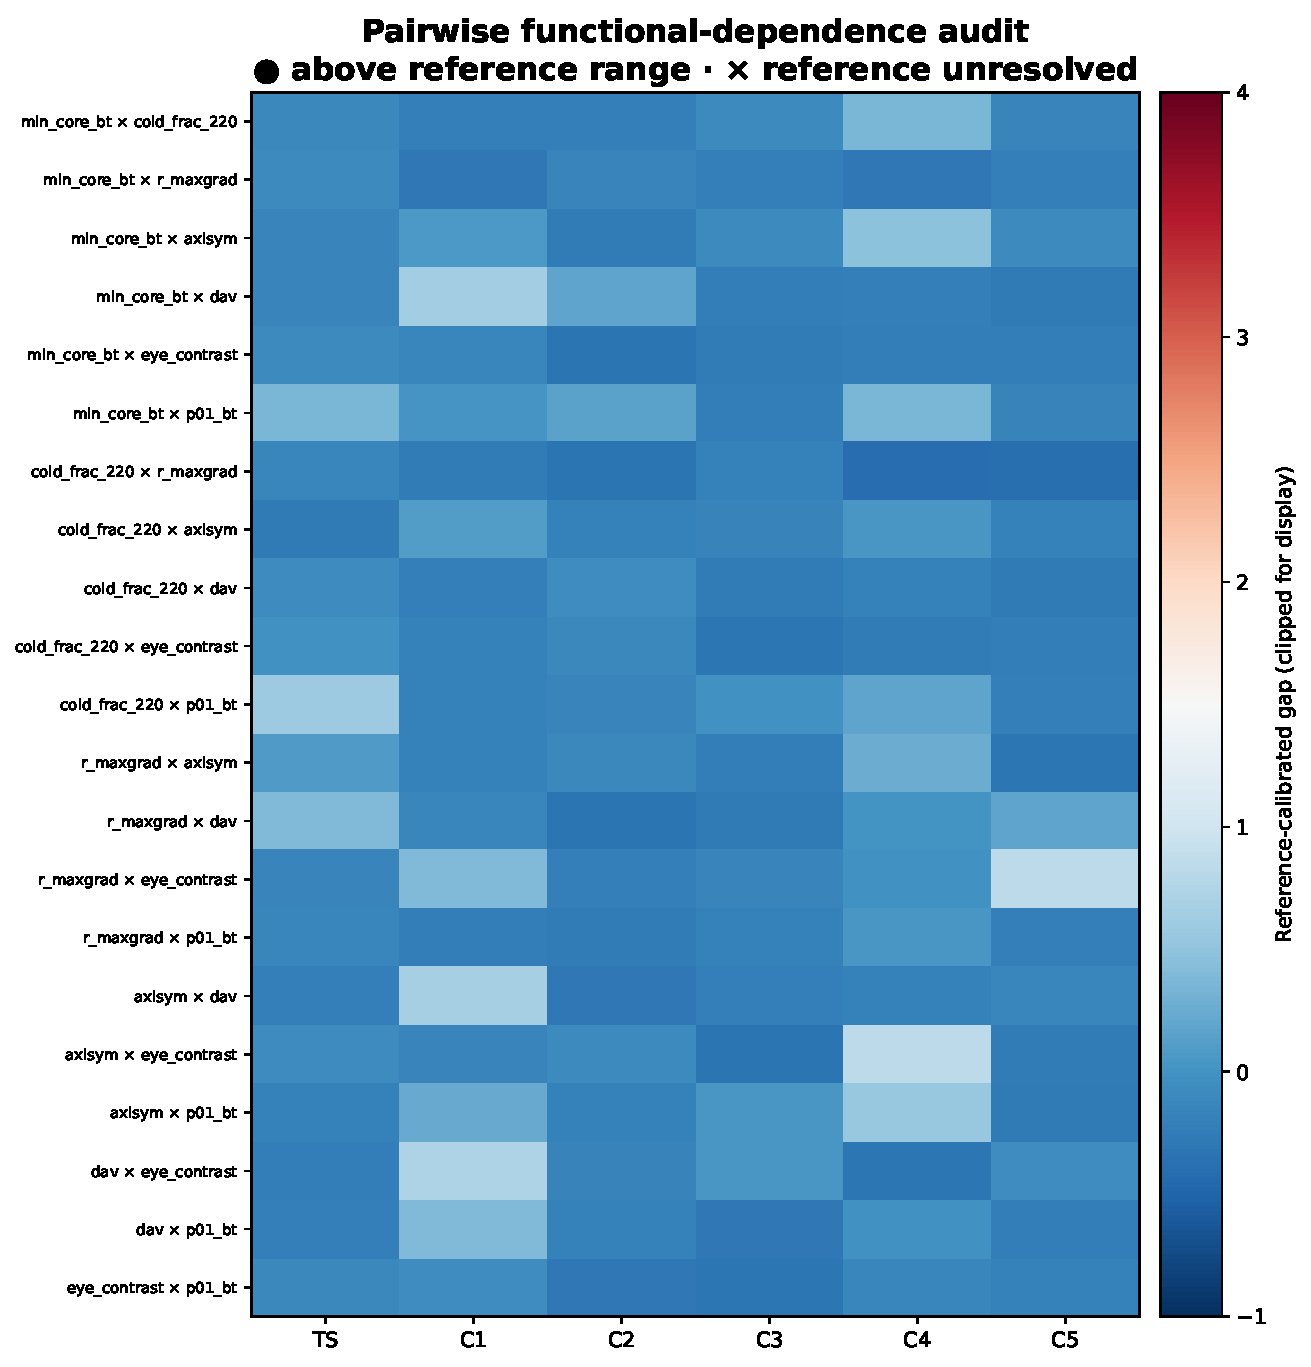
\includegraphics[width=16cm]{figS10.pdf}
\caption{Registered relationships among the physical functionals. These
diagnostics complement, rather than replace, their marginal distributions.}
\label{fig:sdependence}
\end{figure}

\begin{figure}[t]
\centering
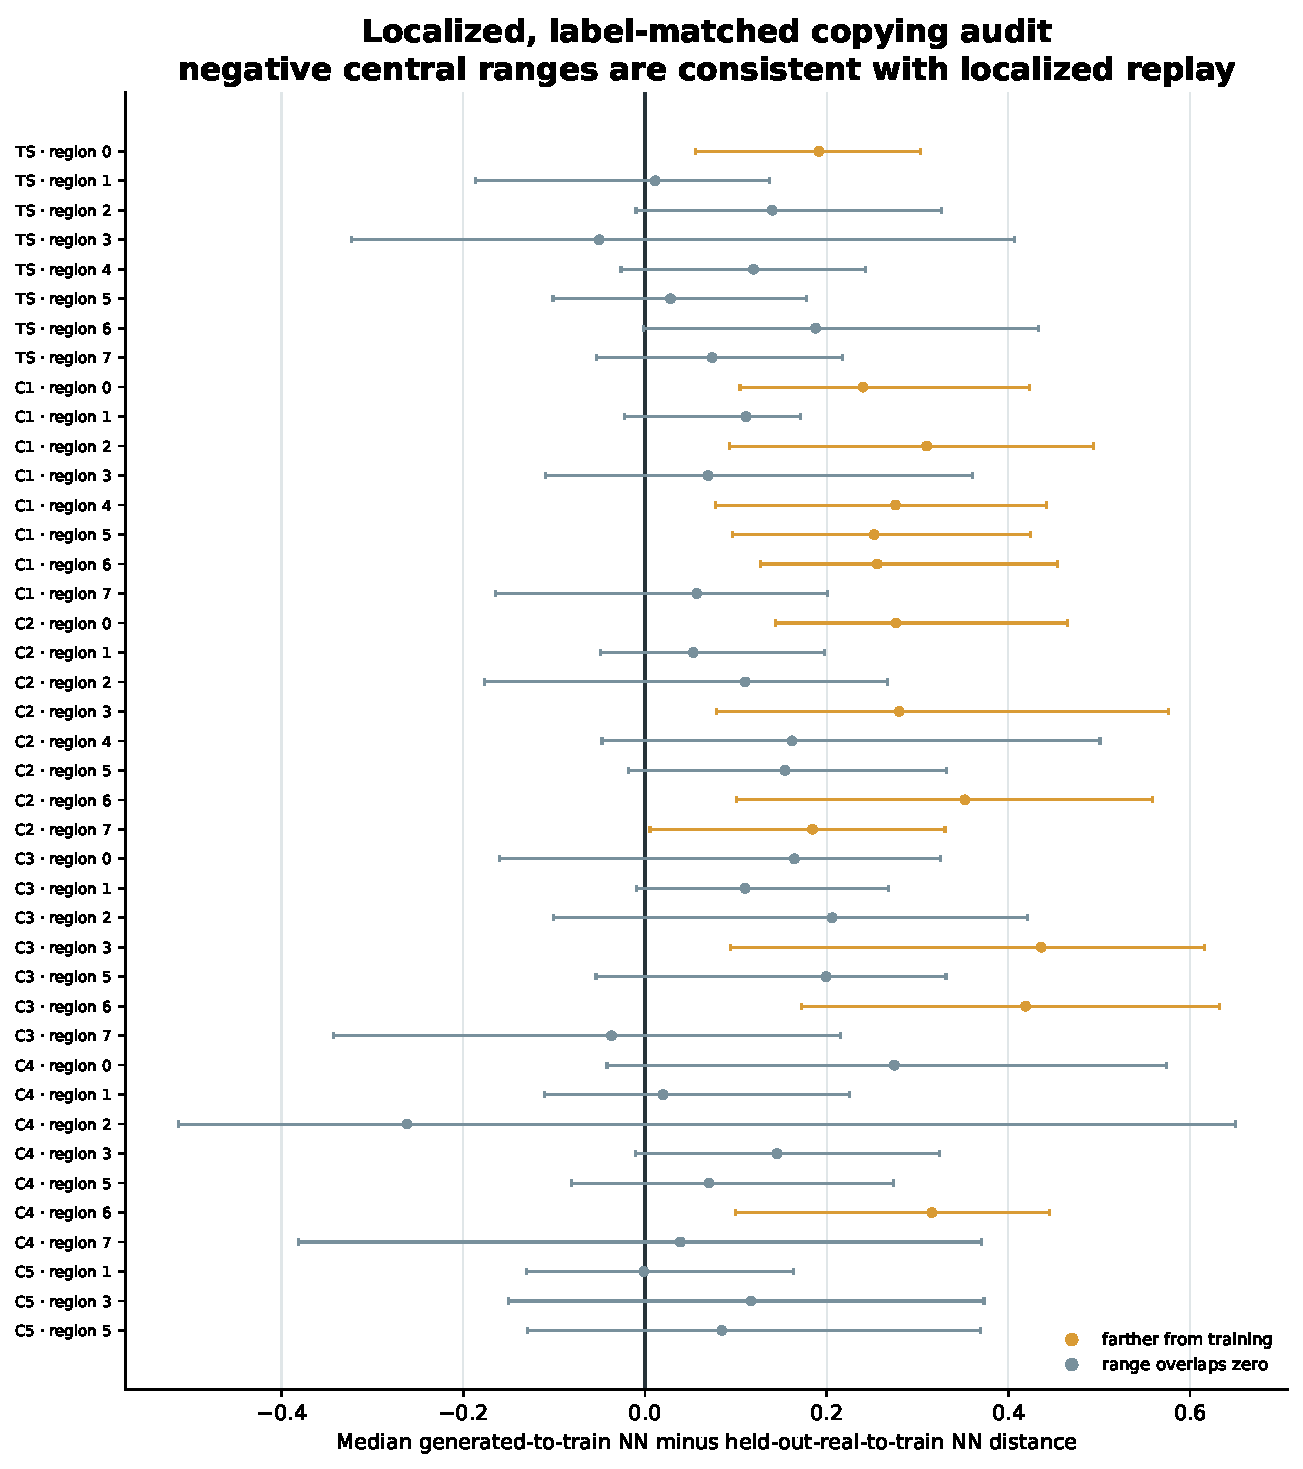
\includegraphics[width=16cm]{figS11.pdf}
\caption{Localized three-sample training-similarity results. Central ranges compare
generated-to-training and held-out-real-to-training nearest-neighbour distances while
resampling generated queries and complete held-out storms.}
\label{fig:smemorization}
\end{figure}

\begin{figure}[t]
\centering
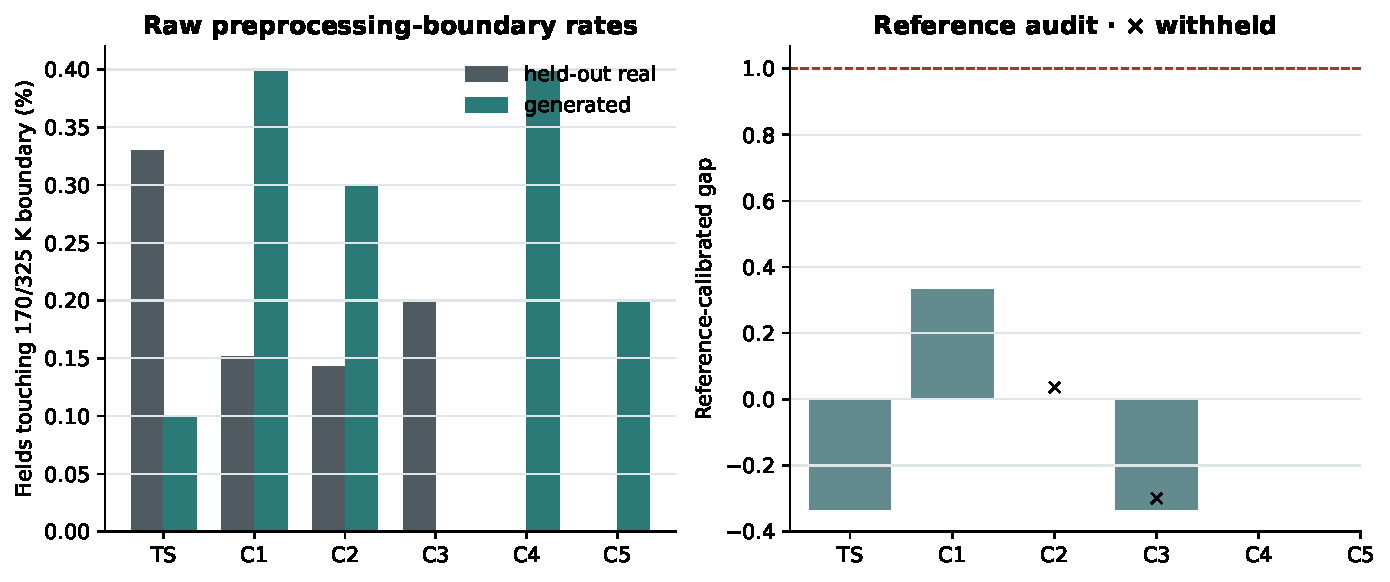
\includegraphics[width=16cm]{figS12.pdf}
\caption{Preprocessing saturation at 170 and 325\,K. The audit identifies mass at
the generator's fixed clipping bounds and makes no claim that these are physical
limits.}
\label{fig:ssaturation}
\end{figure}

\section{Reference stability and synthetic extensions}
\label{sec:sstability}

\begin{figure}[t]
\centering
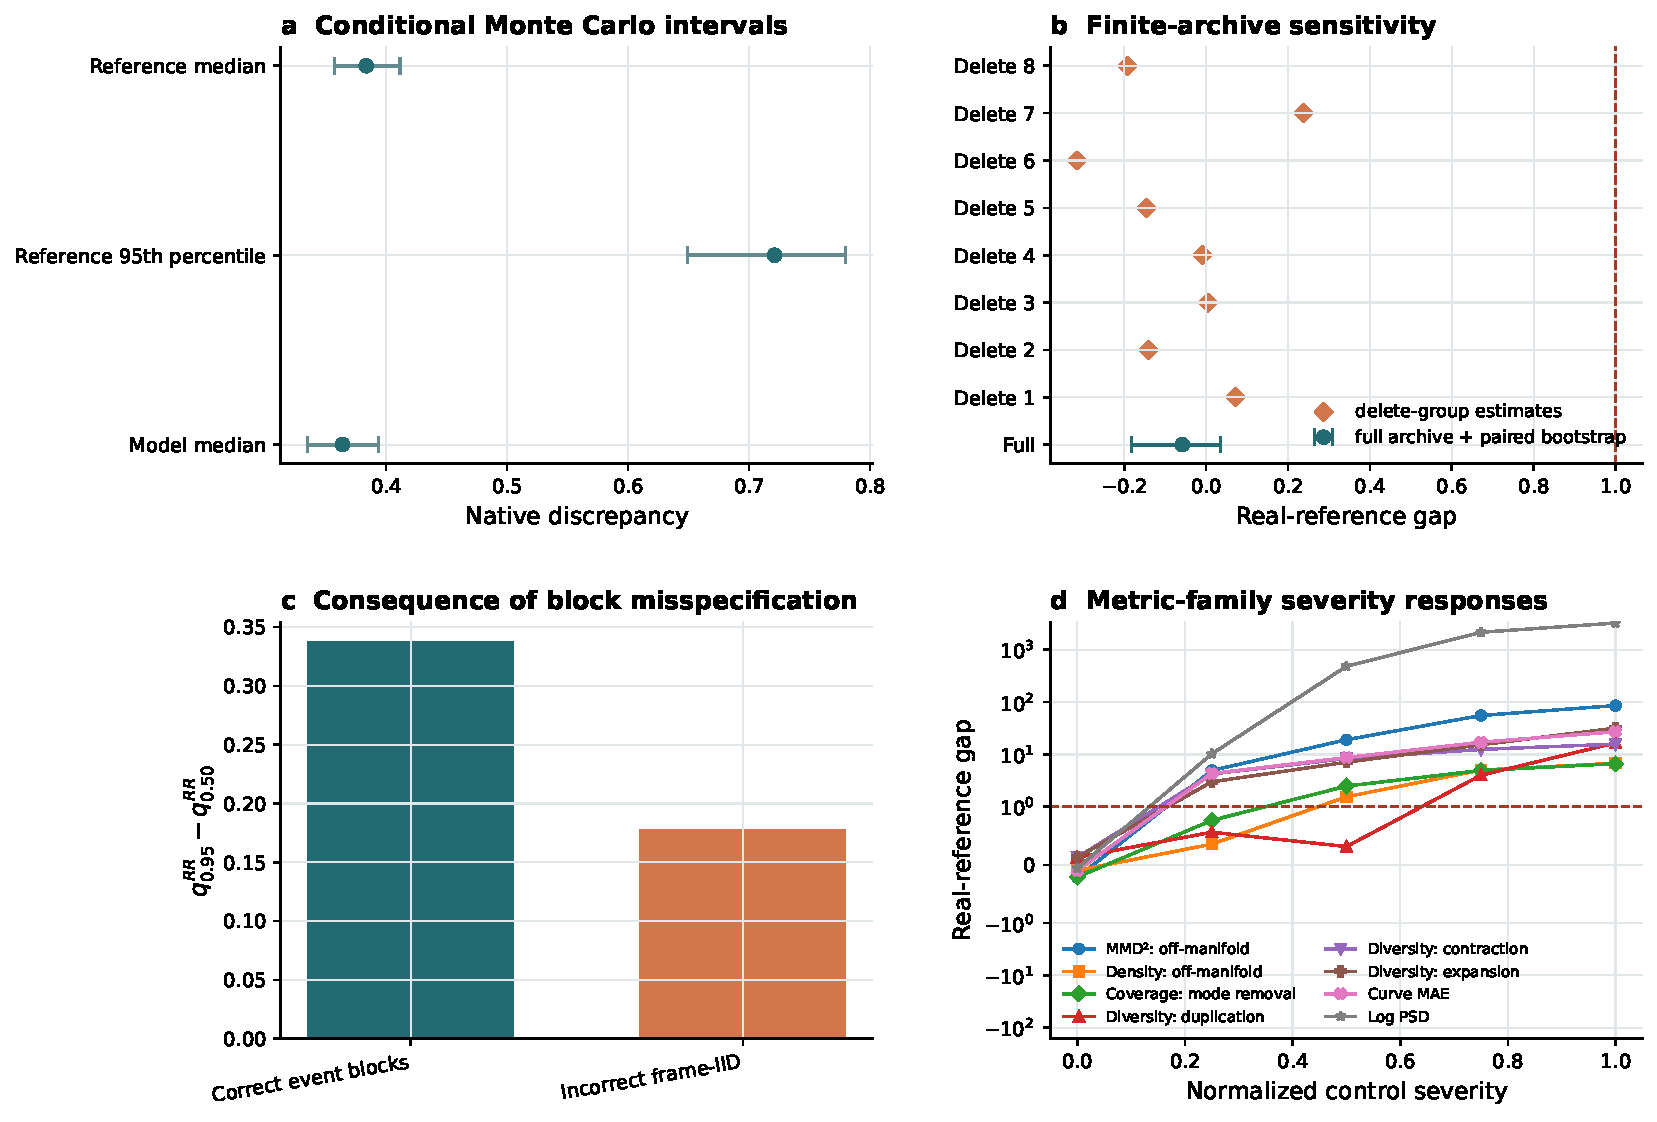
\includegraphics[width=16cm]{figS06.pdf}
\caption{Conditional Monte Carlo intervals for real-reference summaries,
delete-group finite-archive sensitivity, correct event blocking versus intentionally
incorrect frame-IID identifiers, and metric-family severity curves.}
\label{fig:sstability}
\end{figure}

\section{Feature-space robustness}
\label{sec:srobustness}

The registered representation and \FeatureRepresentationVariants{} declared
alternatives produce \FeatureRobustnessComparisons{} class-specific comparisons per
metric. MMD\({}^2\) and coverage remain within the empirical range in
\FeatureMmdWithinCount{} and \FeatureCoverageWithinCount{} comparisons,
respectively. Diversity remains above the range in
\FeatureDiversityAboveCount{}, whereas density does so in
\FeatureDensityAboveCount{}. These are post-hoc robustness summaries rather than a
new model verdict.

\begin{figure}[t]
\centering
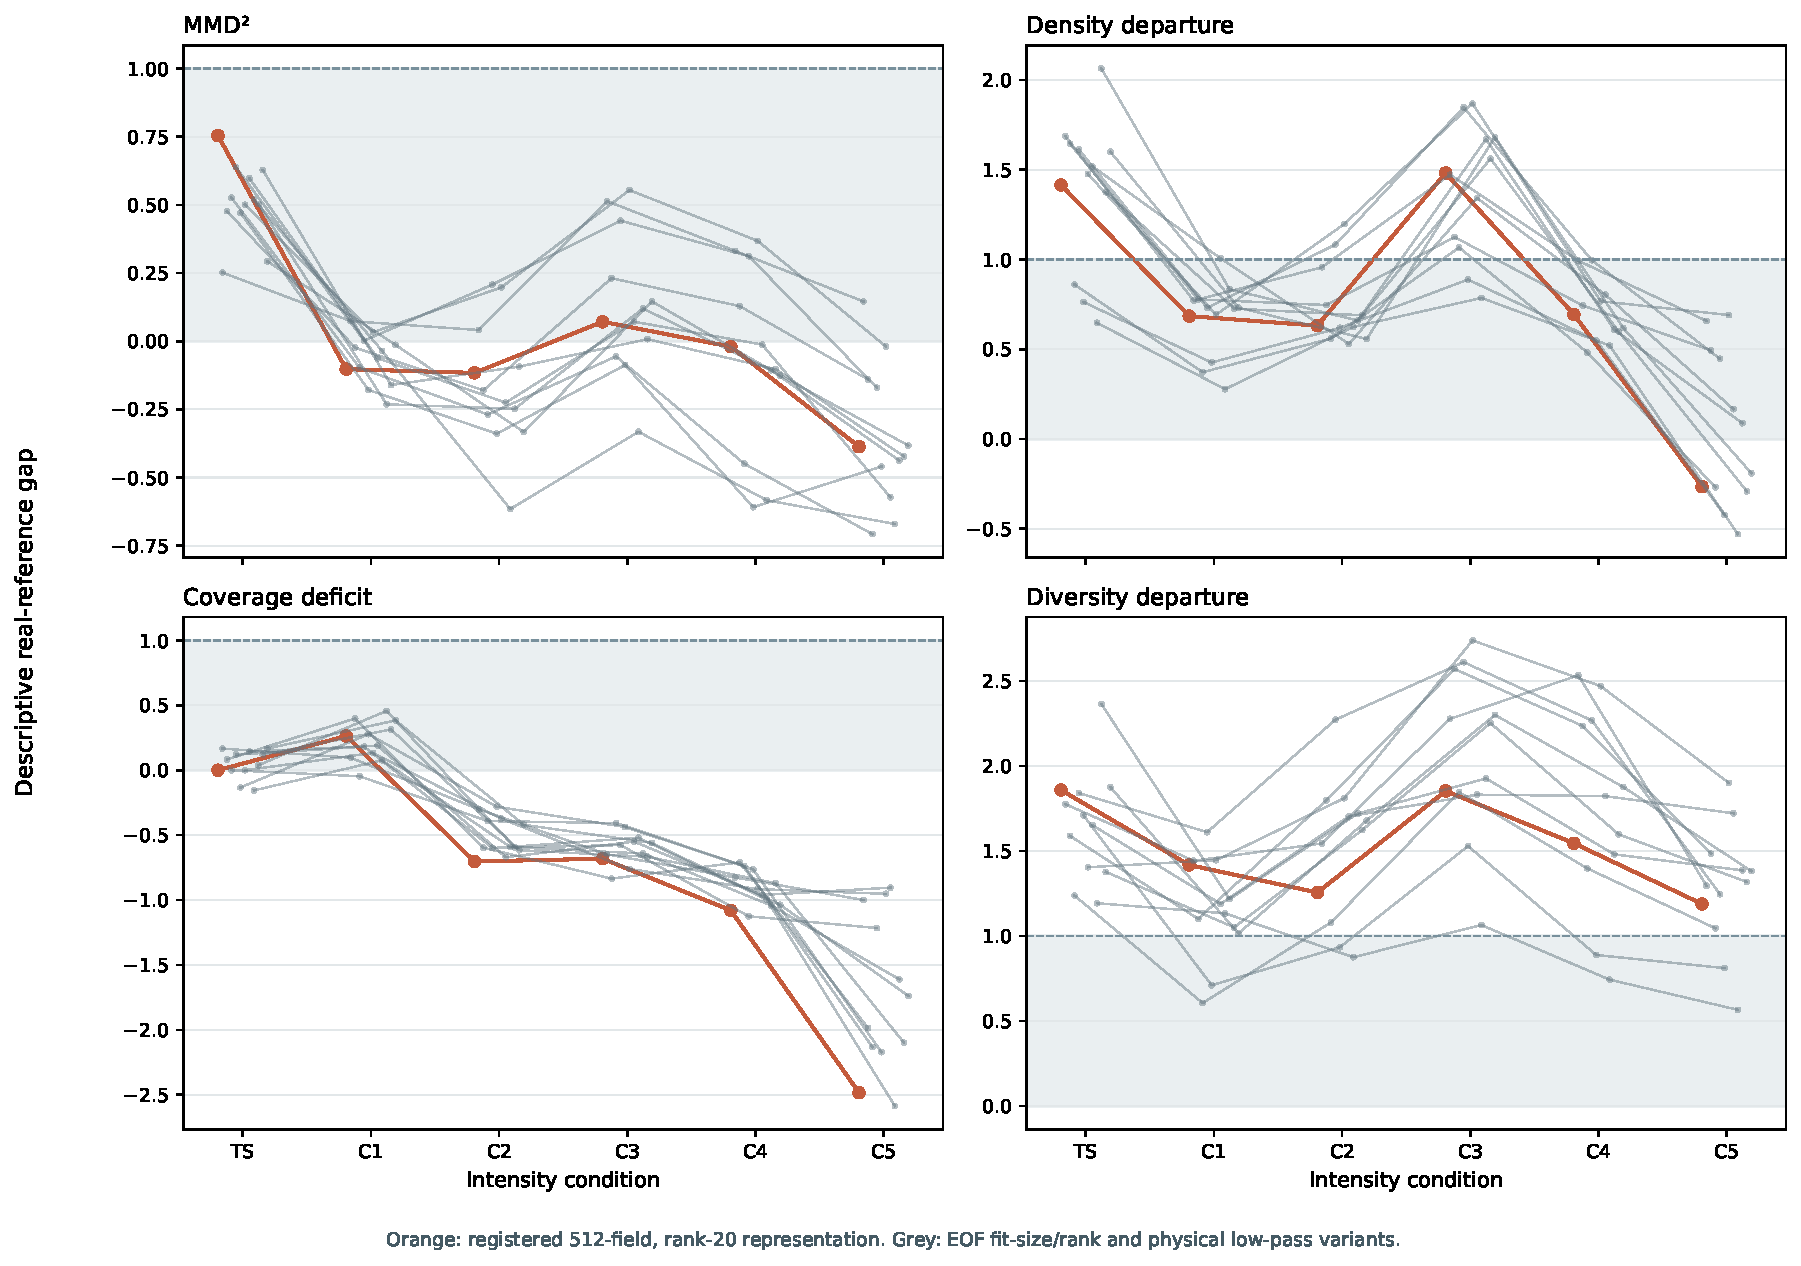
\includegraphics[width=16cm]{figS08.pdf}
\caption{Post-hoc robustness of MMD\({}^2\), density, coverage, and diversity to
EOF fit sizes 256, 512, and 1024; EOF ranks 10, 20, and 40; and declared physical
low-pass scales. The analysis asks whether qualitative patterns persist, weaken, or
reverse across reasonable representations.}
\label{fig:srobustness}
\end{figure}

\section{Continuous-wind response}
\label{sec:swind}

The slope intervals exclude zero in \WindRealResolved{} of
\WindSlopeComparisons{} real-data combinations and \WindGeneratedResolved{} generated
combinations. Both are resolved in \WindBothResolved{} cases, with the same direction
in all \WindBothSameSign{}. \WindCfiveRealResolved{} Category 5 real slopes are
resolved, while
\WindCfiveGeneratedResolved{} generated slopes are; this contrast is reported as a
resolution limitation rather than evidence of disagreement.

\begin{figure}[t]
\centering
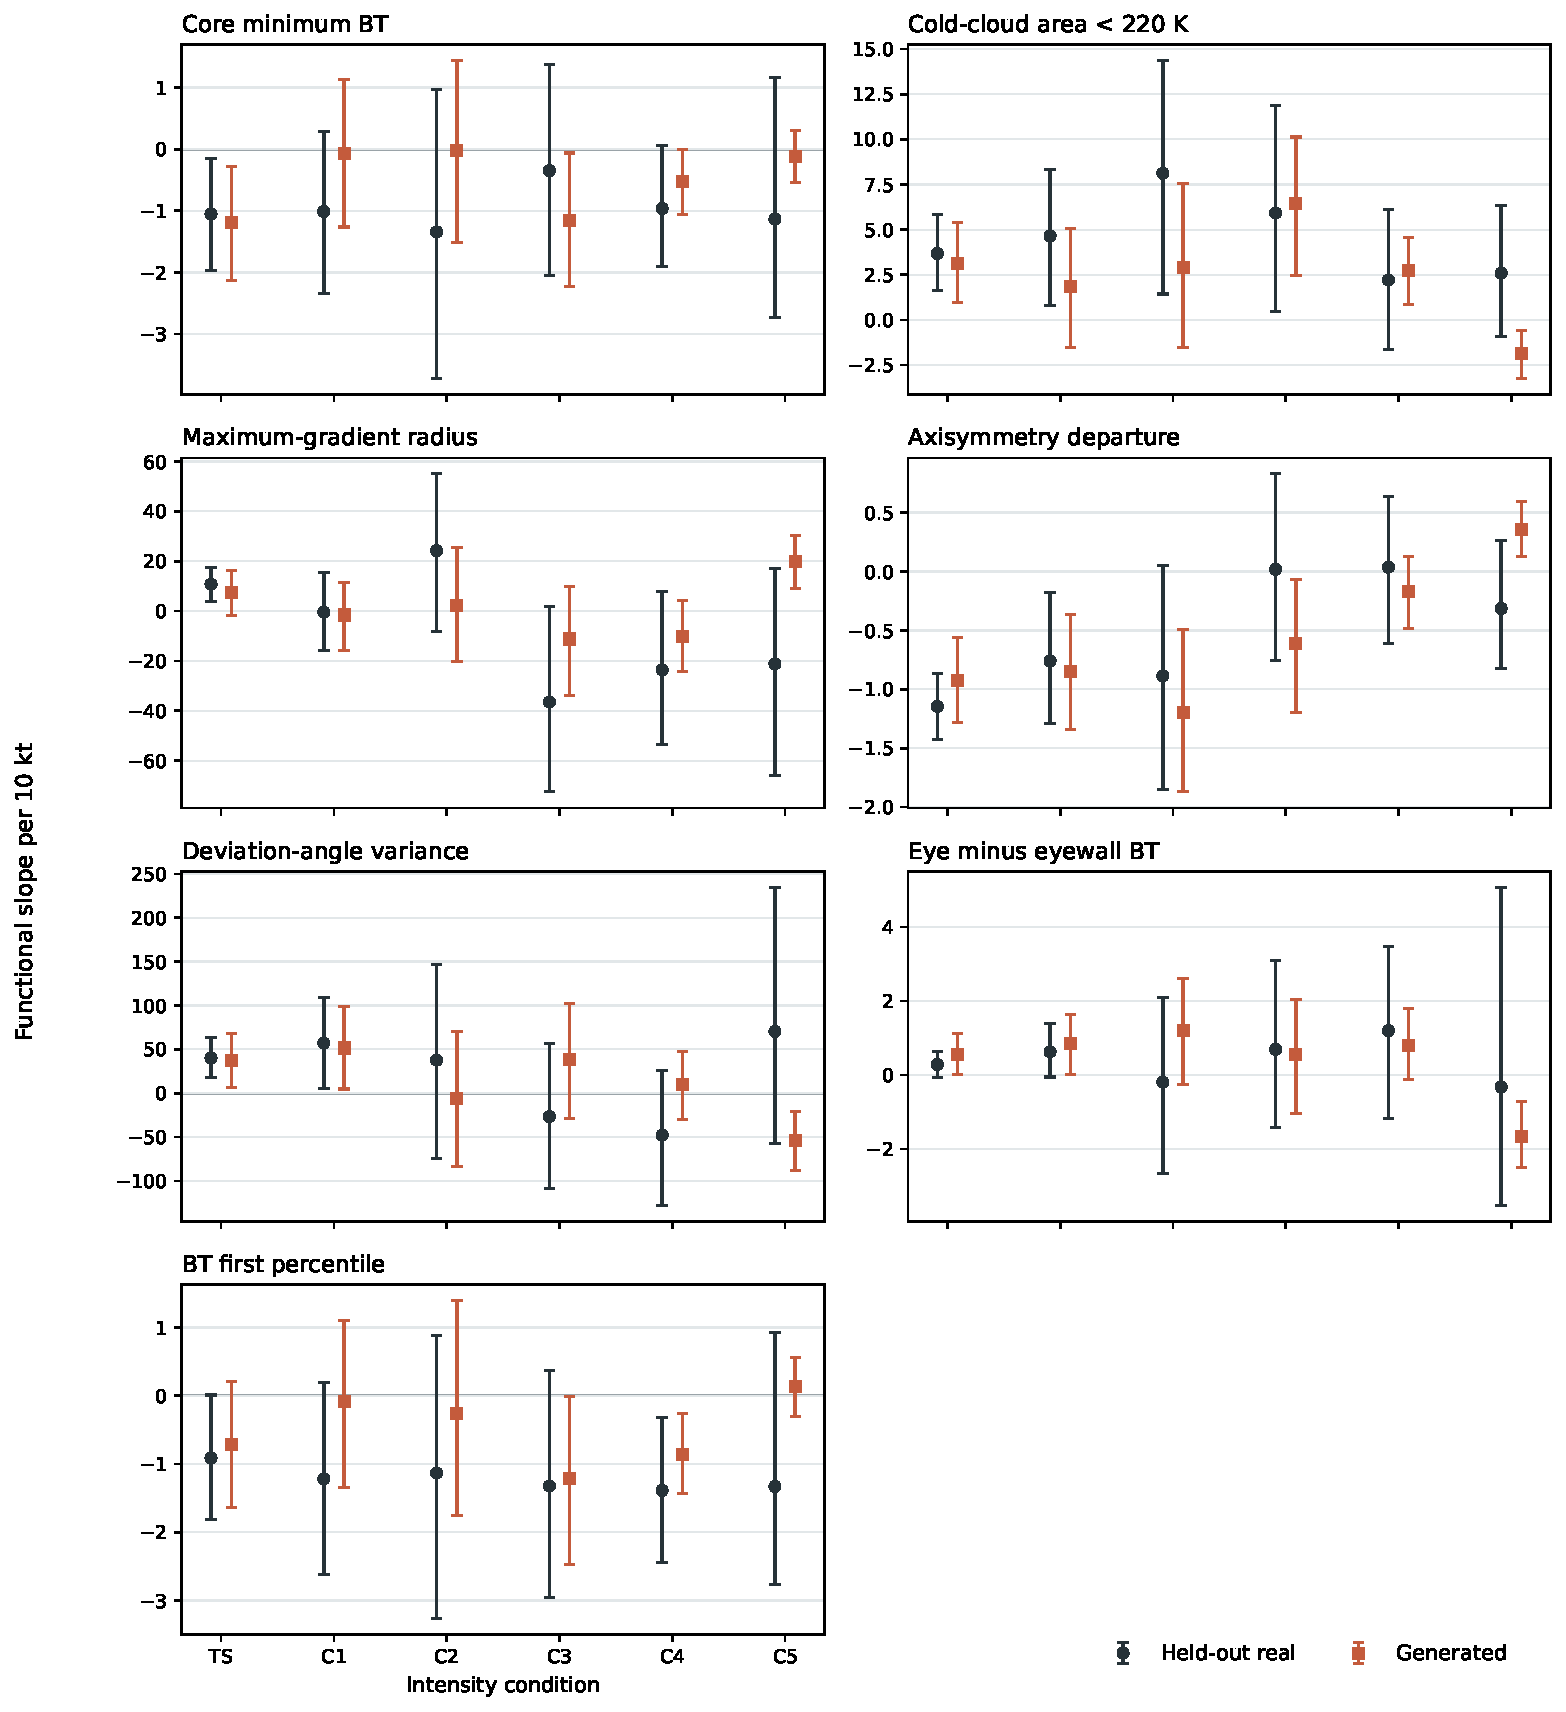
\includegraphics[width=16cm]{figS07.pdf}
\caption{Within-class response of the seven physical quantities to the continuous
wind condition. Real slopes use inverse storm-frequency weights and storm bootstrap
intervals; generated slopes use equal sample weights and sample bootstrap intervals.
The audit is descriptive and carries no equivalence verdict.}
\label{fig:swind}
\end{figure}

\end{document}
